
\documentclass[nototal,handout]{beamer}
\mode<presentation>
{
  \usetheme{Madrid}
  \setbeamercovered{transparent}
}

\usepackage{verbatim}
\usepackage{fancyvrb}
\usepackage[english]{babel}
\usepackage[latin1]{inputenc}
\usepackage{times}
\usepackage{tikz}
\usepackage[T1]{fontenc}
\usepackage{graphicx} %sjr added
\usepackage{subfigure} %crs added
\graphicspath{{figures/}}
\usepackage{hyperref}

\author[Schmidt]{Charles R. Schmidt}
\institute[SDSU]{Department of Geography\\San Diego State University}
\title[Irregular Topology in Spherical-SOM]{Effects of Irregular Topology in Spherical Self-Organizing Maps}
\subtitle{Thesis presentation}
\date[Thesis]{September 15, 2008}

% Delete this, if you do not want the table of contents to pop up at
% the beginning of each subsection:
\AtBeginSubsection[]
{
  \begin{frame}<beamer>
    \frametitle{Outline}
    \tableofcontents[currentsection,currentsubsection]
  \end{frame}
}


% If you wish to uncover everything in a step-wise fashion, uncomment
% the following command: 
\beamerdefaultoverlayspecification{<+->}
\begin{document}
\begin{frame}
  \titlepage
\end{frame}
\begin{frame}
  \frametitle{Outline}
  \tableofcontents[pausesections]
  % You might wish to add the option [pausesections]
\end{frame}



\section{Background} 

\subsection{The Self-Organizing Map} 

\begin{frame}
	\frametitle{The Self-Organizing Map}
 
\begin{block}{What is the SOM}
 \begin{itemize}
 \item  Artificial Neural Network
 \item  High Dimension Input Data
 \item  Unsupervised Competitive Learning Process
 \item  Each Neuron Models of a Portion of the Input Space
 \end{itemize}
 \end{block} 
\begin{block}{Applications}
 \begin{itemize}
 \item  Data Visualization
 \item  Data Reduction
 \item  Clustering
 \end{itemize}
 \end{block} \end{frame} 

\begin{frame}
	\frametitle{In Terms of Geography (Skupin 2004)}
  \begin{center}
  \begin{figure}
  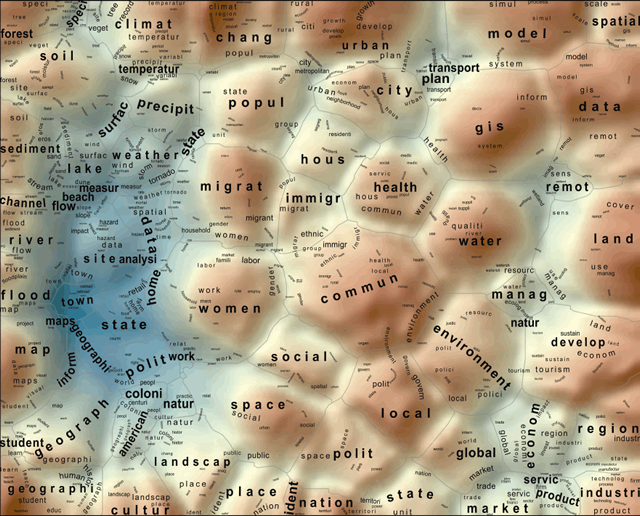
\includegraphics[width=.8\linewidth]{skupin.png}
  \end{figure}
  \end{center}
 \end{frame} 

\begin{frame}
	\frametitle{SOM as Dimensionality Reduction}
  \begin{center}
  \begin{figure}
  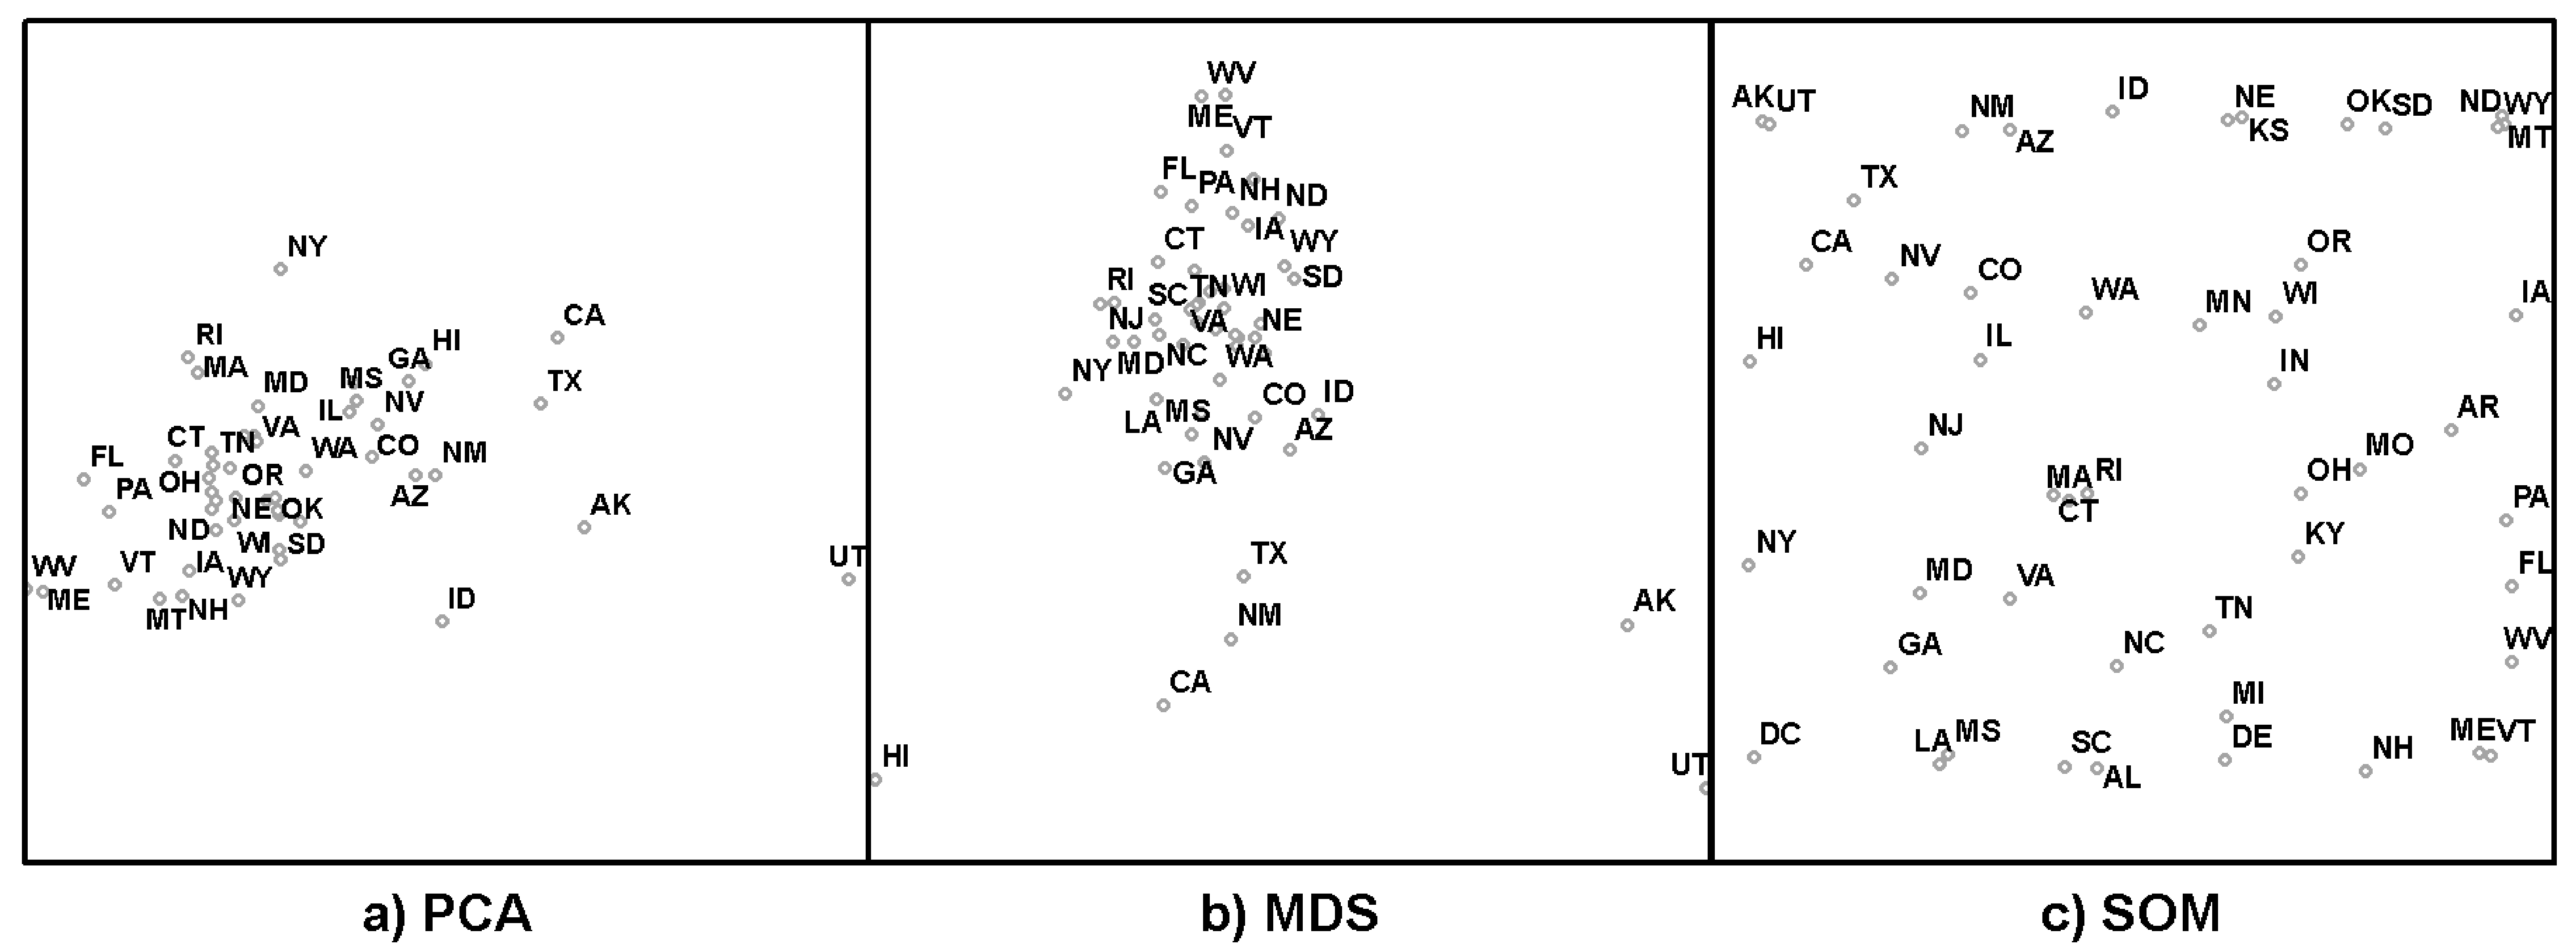
\includegraphics[width=0.90\linewidth]{dimensionReduction.png}
  \end{figure}
  \end{center}
  \vspace{1in} (Skupin 2008)
 \end{frame} 

\begin{frame}
	\frametitle{SOM as Clustering}
  \begin{center}
  \begin{figure}
  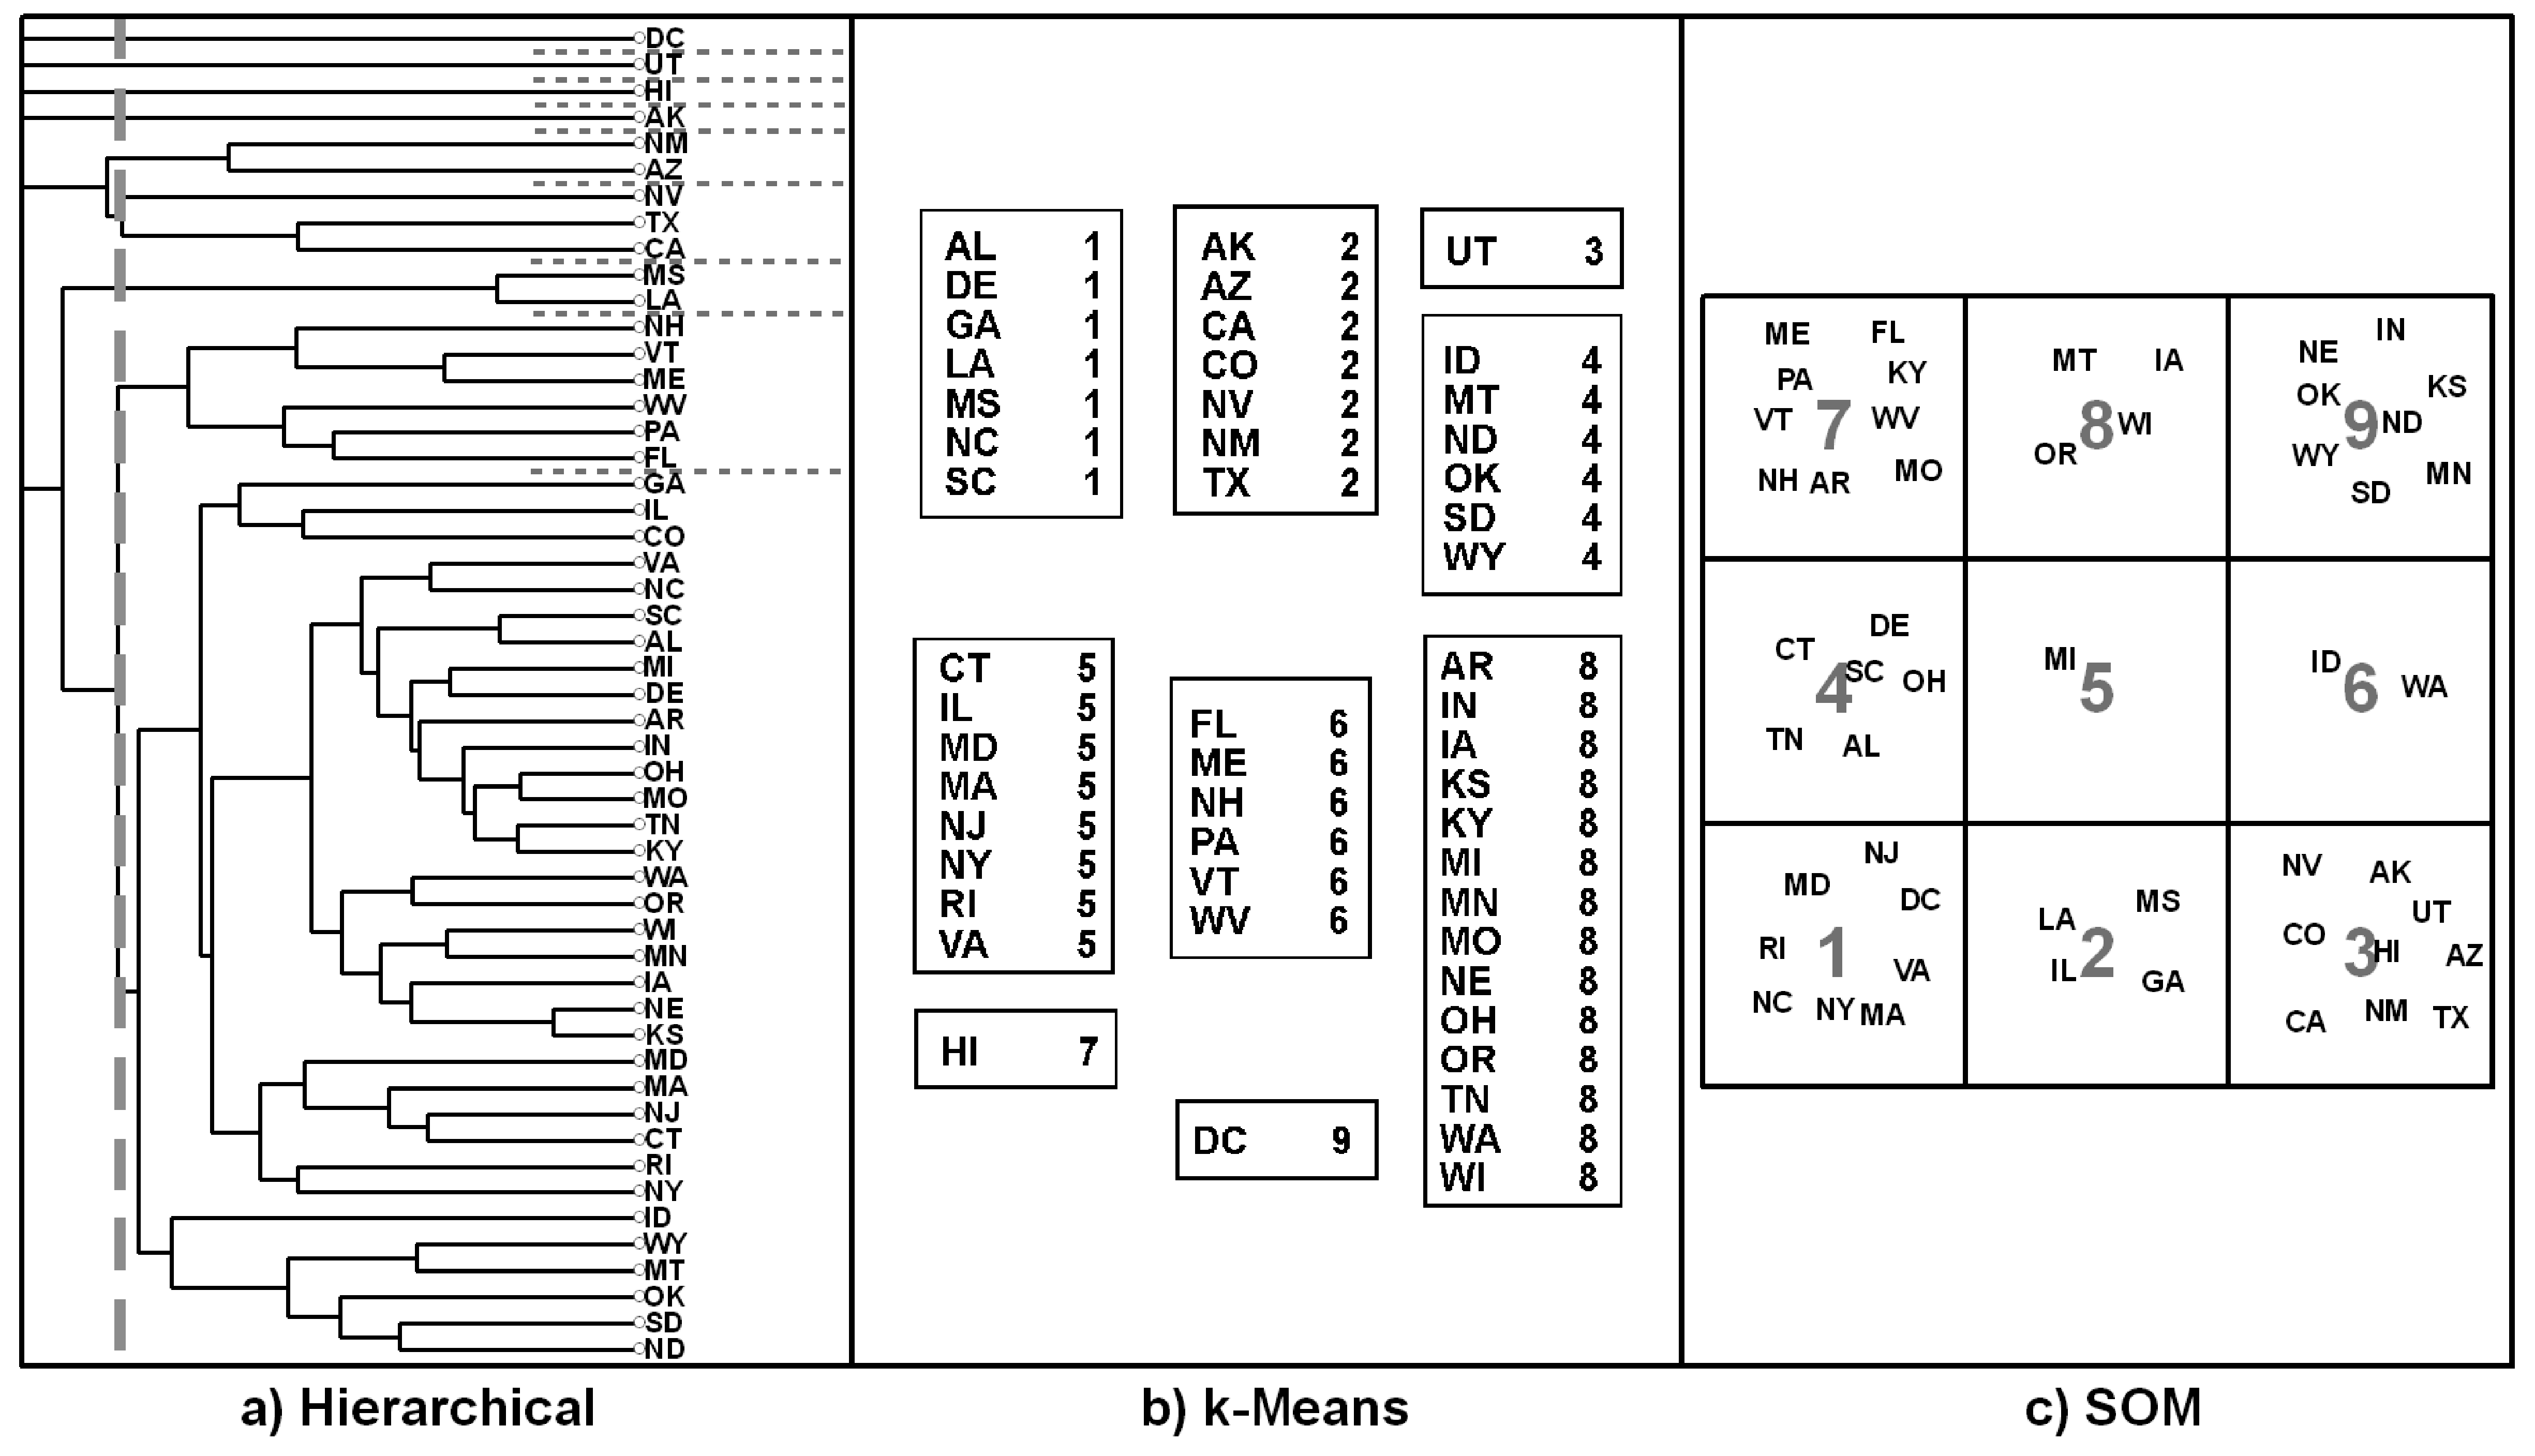
\includegraphics[width=0.90\linewidth]{clustering.png}
  \end{figure}
  \end{center}
  (Skupin 2008)
 \end{frame} 

\begin{frame}
	\frametitle{SOM as Clustering}
  \begin{center}
  \begin{figure}
  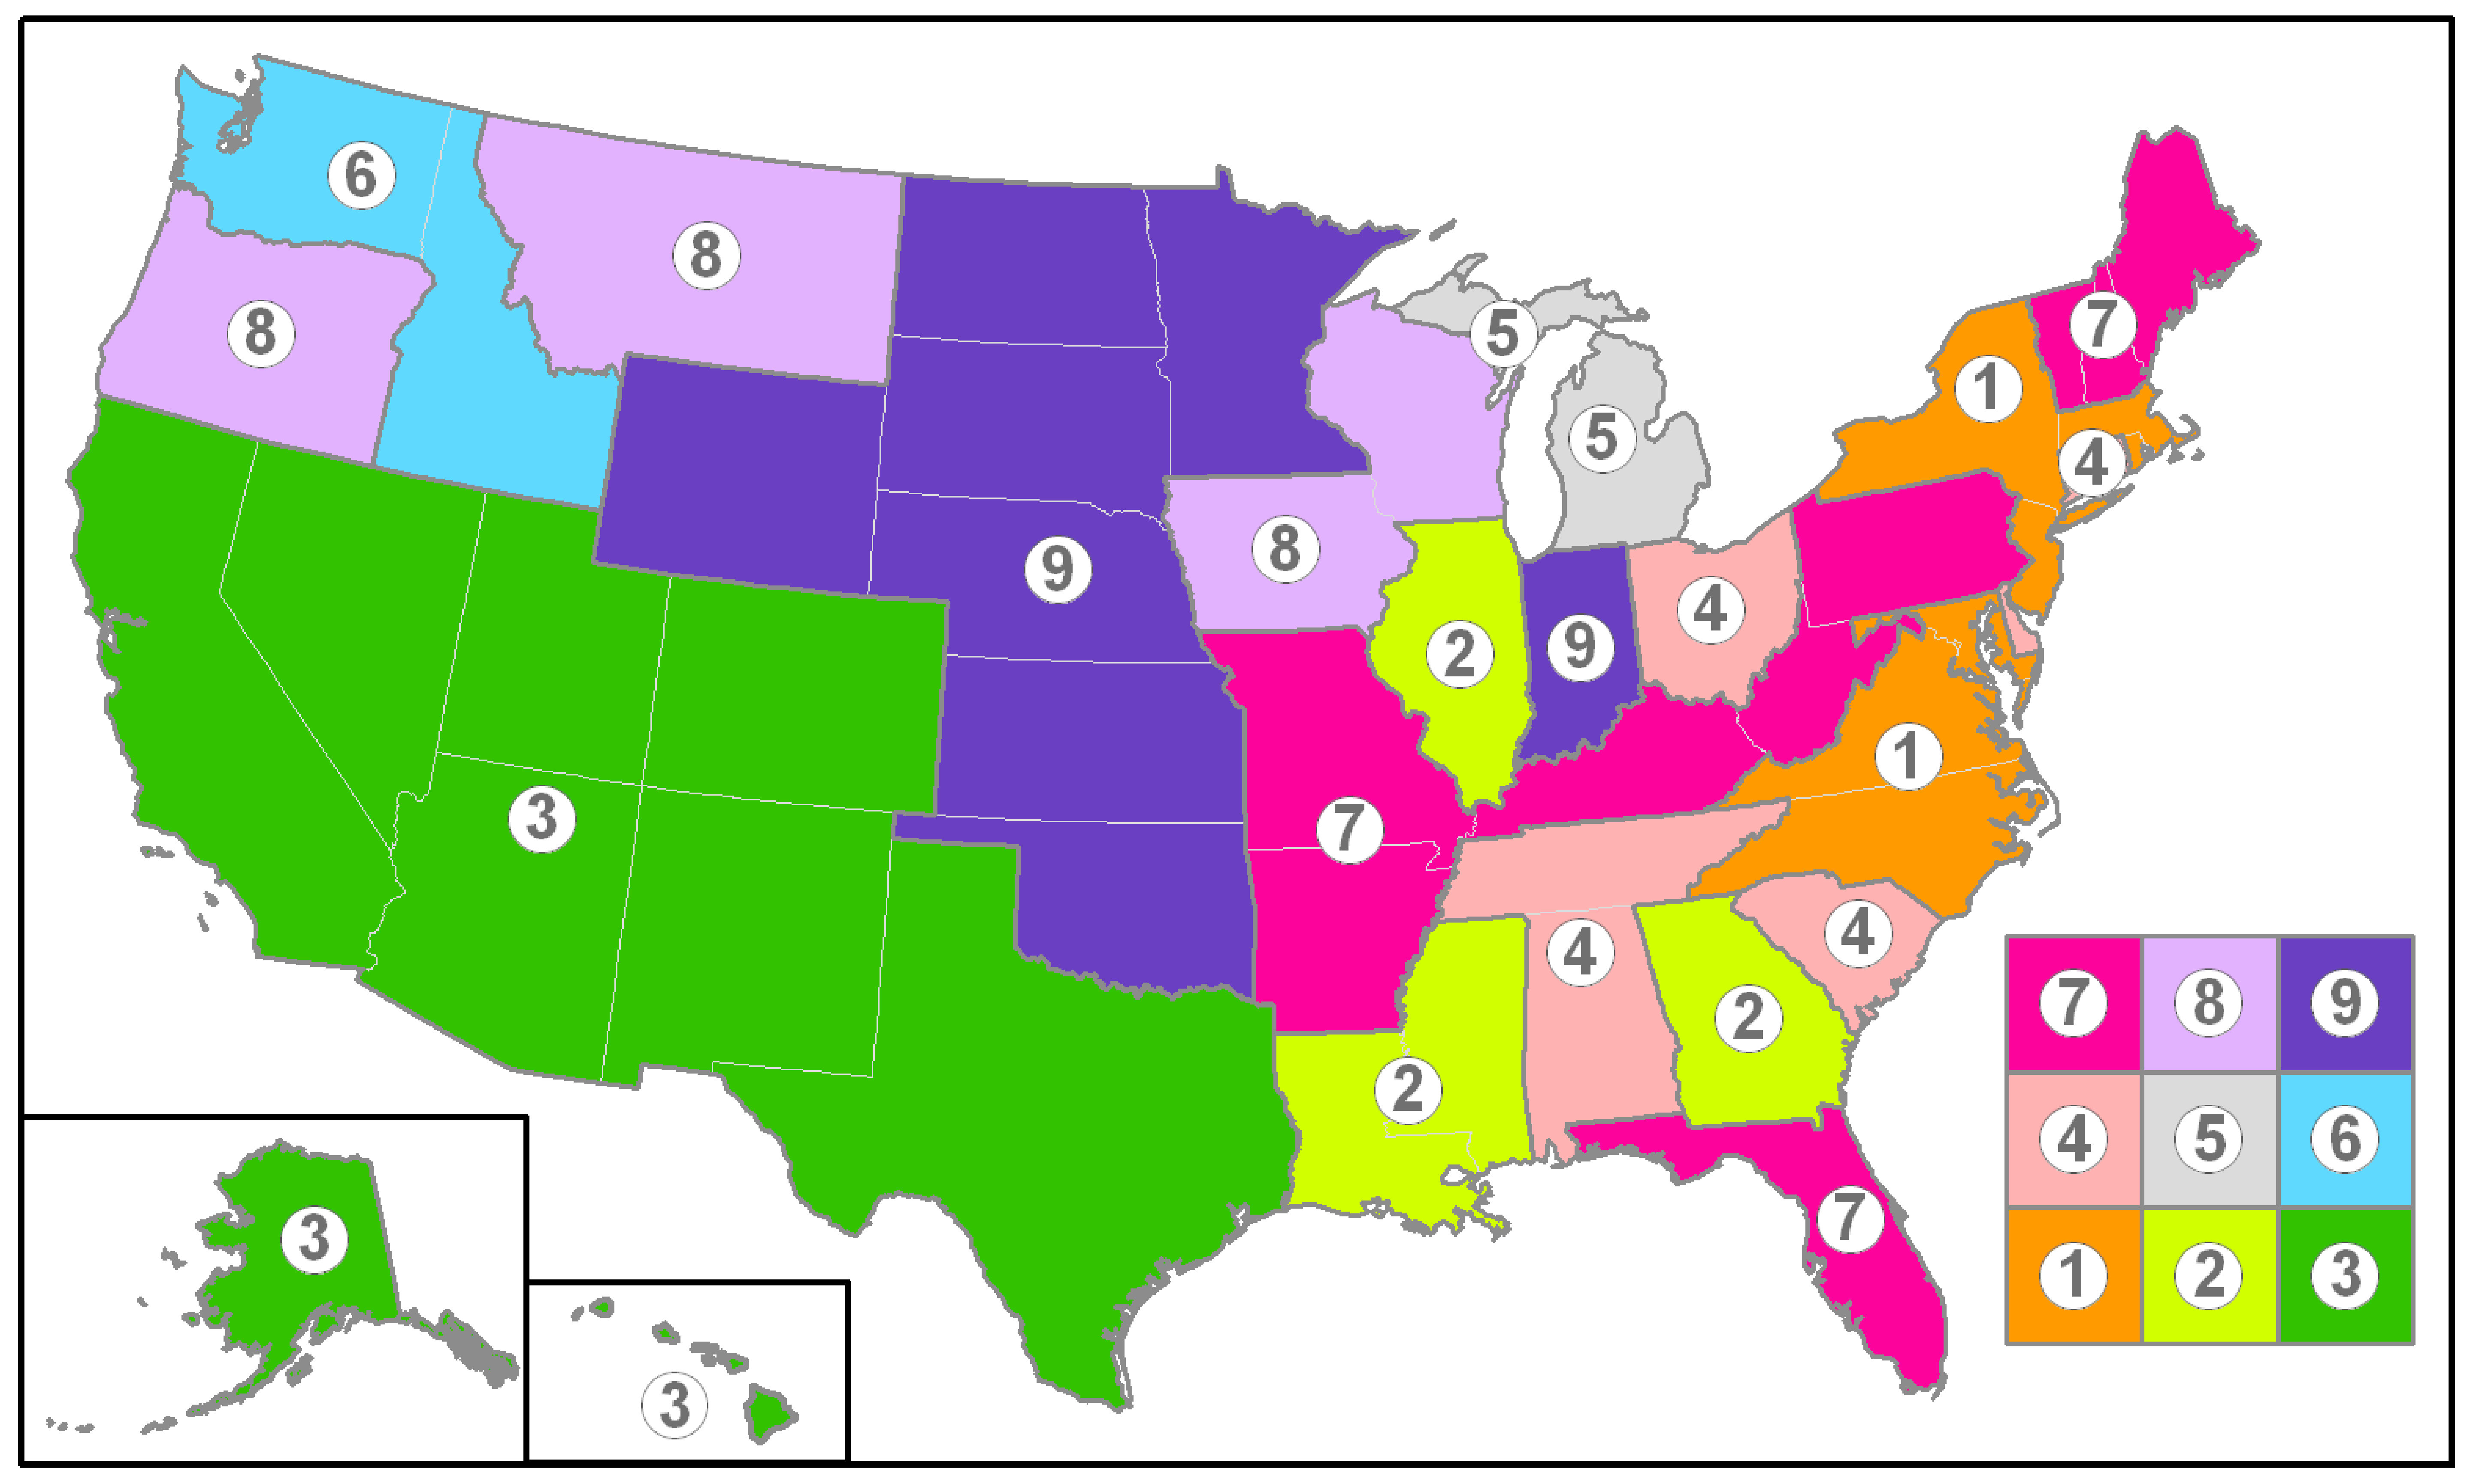
\includegraphics[width=0.90\linewidth]{clustermap.png}
  \end{figure}
  \end{center}
  (Skupin 2008)
 \end{frame} 

\begin{frame}
	\frametitle{SOM and GIScience}
  \begin{center}
  \begin{figure}
  
\includegraphics[width=0.50\linewidth]{book.png}
  \end{figure}
  \end{center}
 \end{frame} 

\begin{frame}
	\frametitle{SOM and GIScience}
  \begin{quote}
  "translate \emph{data similarities} into \emph{spatial relationship}" 
  \end{quote}
  \hspace{2in} -- Helge Ritter, 1999
 \end{frame} 

\begin{frame}
	\frametitle{Training}
 
\begin{block}{Assignment and Updating}
  \begin{center}
  \begin{figure}
  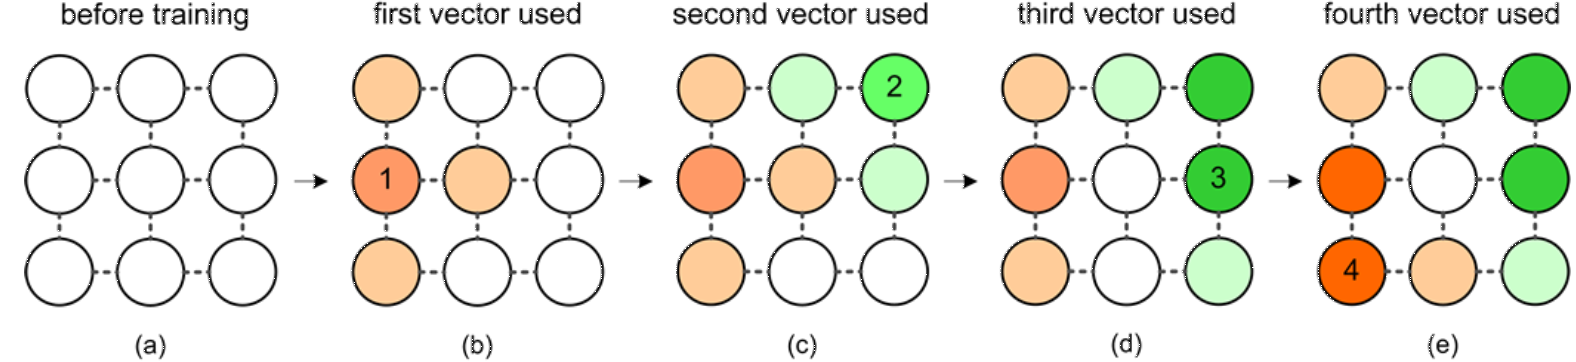
\includegraphics[width=0.90\linewidth]{input.png}
  \end{figure}
  \end{center}
 \end{block} \end{frame} 

\begin{frame}
	\frametitle{Training}
 
\begin{block}{Training}
 \begin{itemize}
 \item  Randomize input vectors
 \item  Randomly Initialize the neurons
 \item  Loop Until Map Converges
 \begin{itemize}
 \item  Grab an Input Vector
 \item  Find the Best Matching Neuron and its Neighborhood
 \item  Modify the Weights of the Neurons to Make them More Similar to the Input Vector
 \end{itemize}
 \end{itemize}
 \end{block} \end{frame} 

\begin{frame}
	\frametitle{Training}
 
\begin{block}{Iterations}
  \begin{center}
  \begin{figure}
  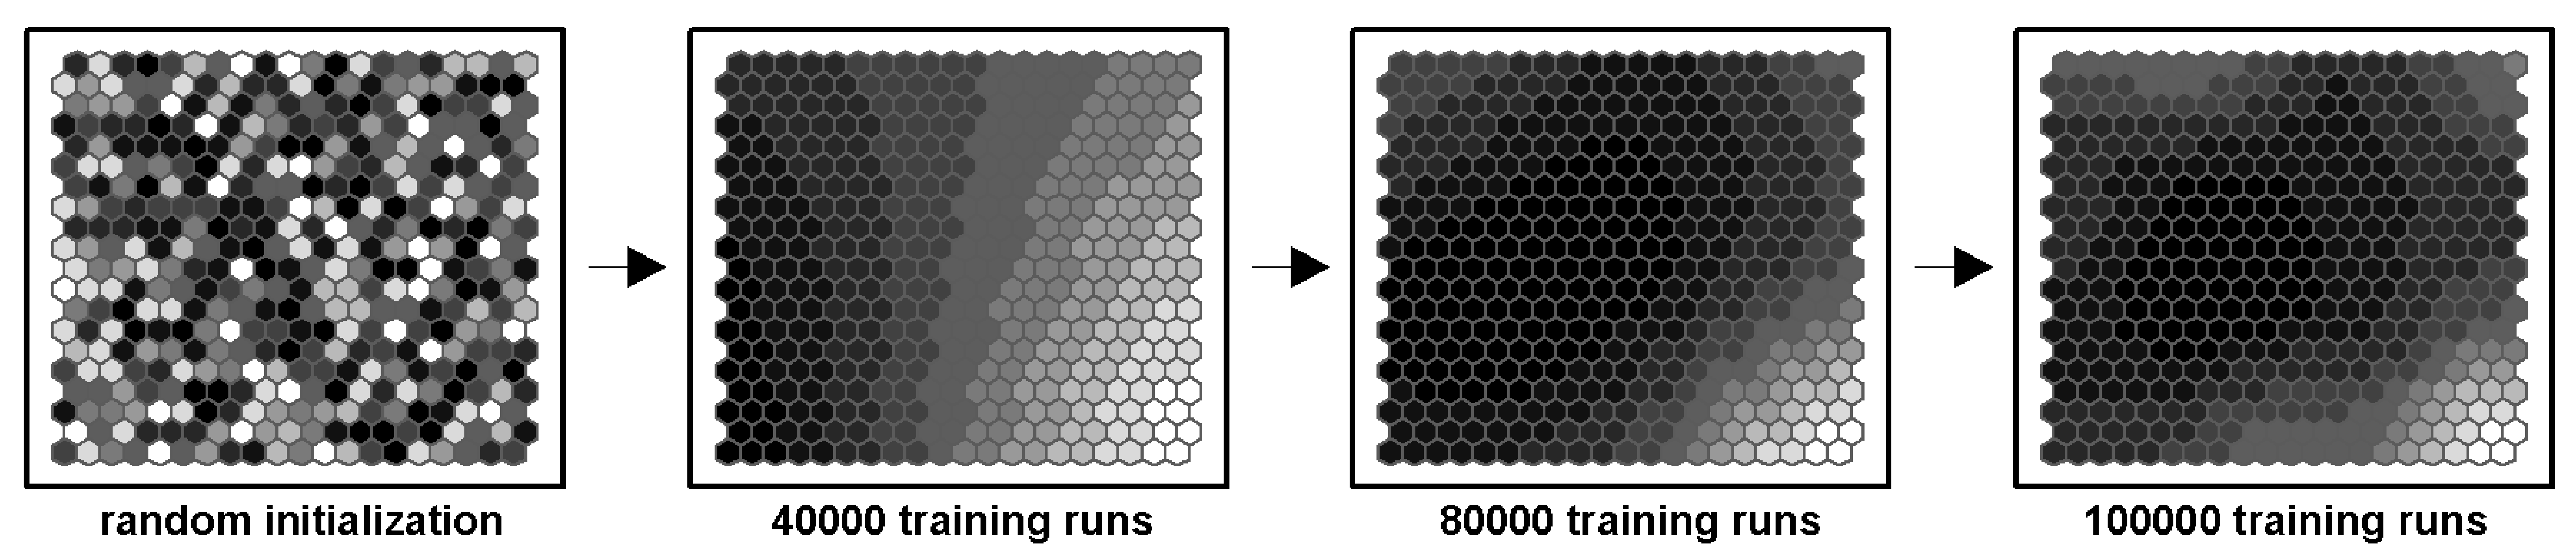
\includegraphics[width=0.90\linewidth]{somtrain.png}
  \end{figure}
  \end{center}
 \end{block} \end{frame} 

\subsection{Edge Effects in SOM} 

\begin{frame}
	\frametitle{Edge Effects in SOM}
  \begin{center}
  \begin{figure}
  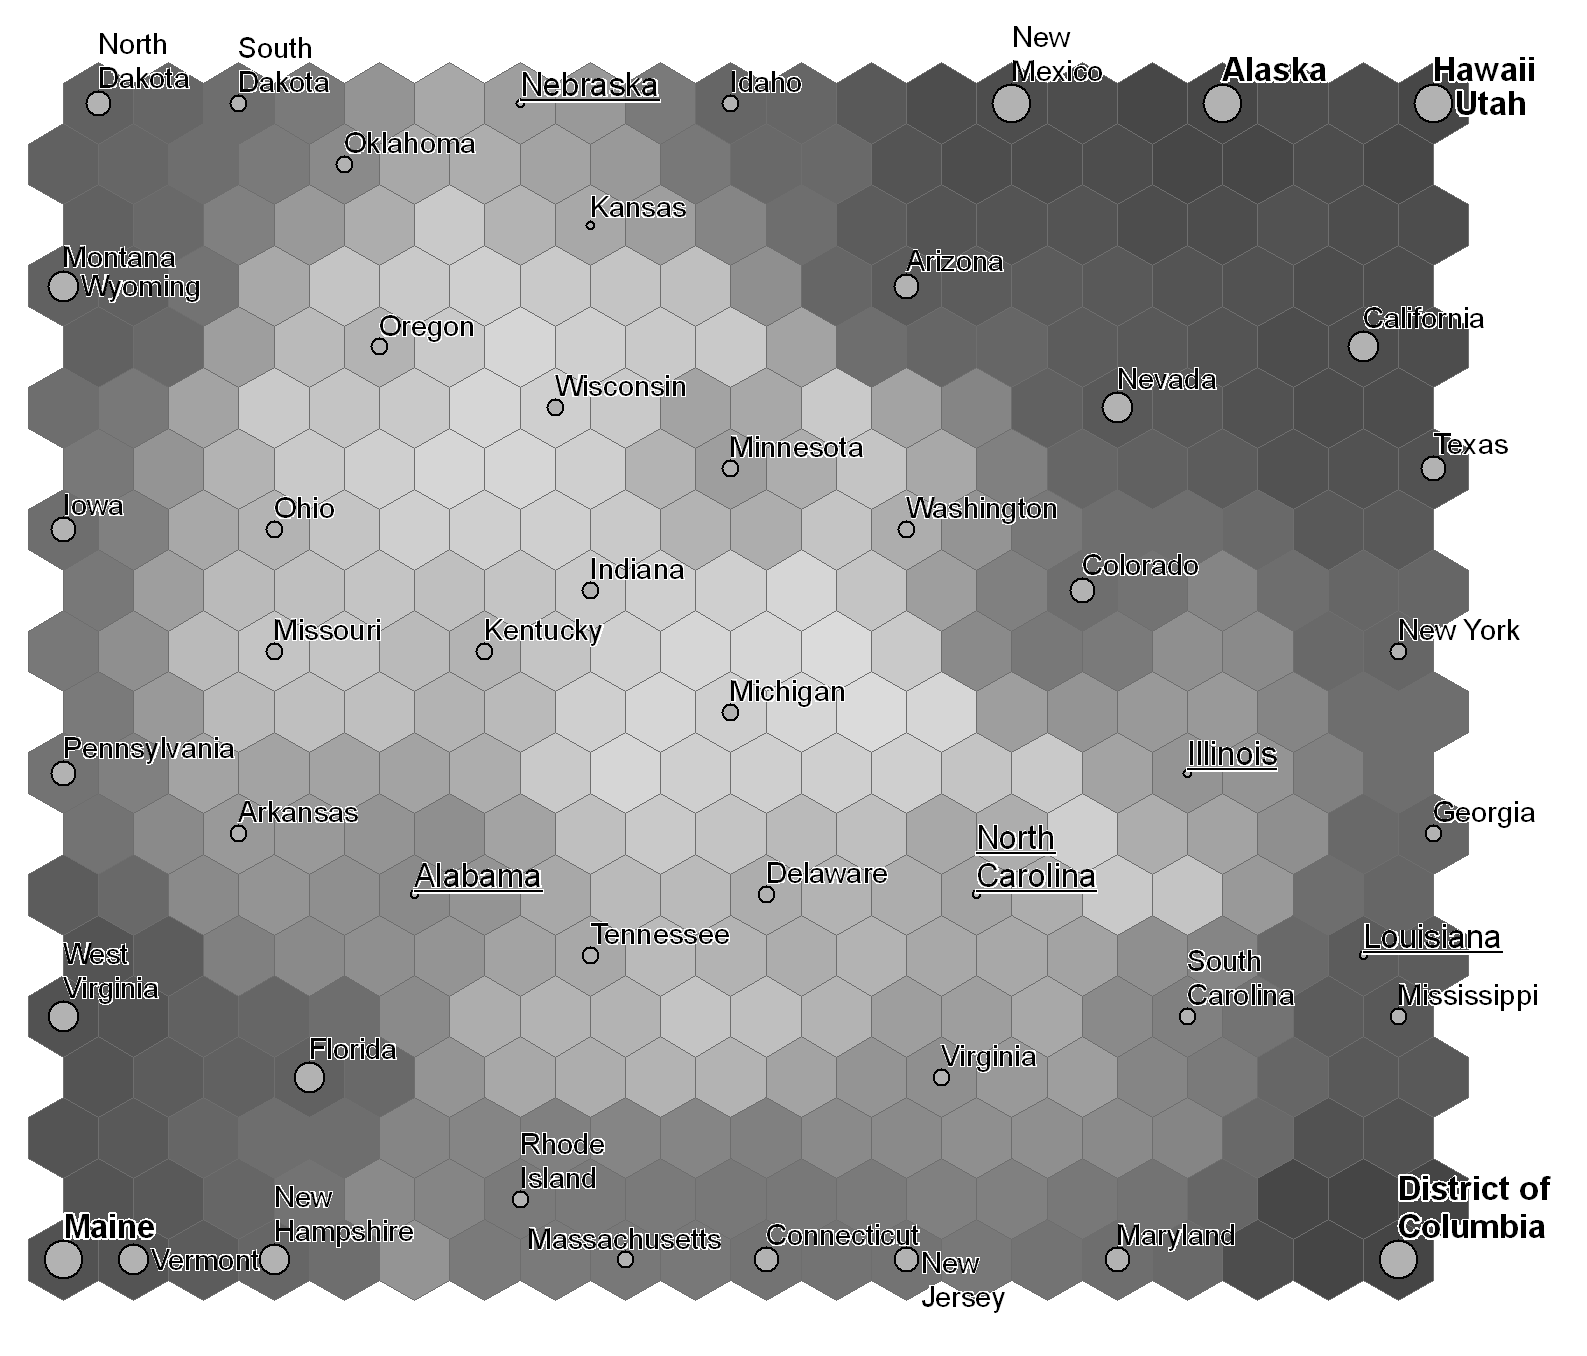
\includegraphics[width=0.60\linewidth]{gridedge.png}
  \end{figure}
  \end{center}
 \end{frame} 

\begin{frame}
	\frametitle{Edge Effects}
 
\begin{block}{In SOM}
 \begin{itemize}
 \item  Higher density of observations mapped to edge neurons
 \item  Higher internal heterogeneity for edge neurons
 \end{itemize}
 \end{block} 
\begin{block}{In Spatial Analysis}
 \begin{itemize}
 \item  Inflated nearest neighbor distances
 \item  Mask the true distribution
 \end{itemize}
 \end{block} 
\begin{block}{Components of Edge Effect}
 \begin{itemize}
 \item  True Boundary
 \end{itemize}
 \end{block} \end{frame} 

\begin{frame}
	\frametitle{Suggested Solutions}
 
\begin{block}{With Edges}
 \begin{itemize}
 \item  Hierarchical SOM
 \item  Growing SOM
 \item  Mathematical Weighting
 \end{itemize}
 \end{block} 
\begin{block}{Without Edges}
 \begin{itemize}
 \item  Spherical SOM
 \item  Toroidal SOM
 \end{itemize}
 \end{block} \end{frame} 

\begin{frame}
	\frametitle{Spherical SOM}
 
\begin{block}{Geodesic}
 \begin{itemize}
 \item  Most Common
 \item  Highly Regular
 \item  Limited Network Size
 \end{itemize}
 \end{block} 
\begin{block}{Rakhmanov (Spherical)}
 \begin{itemize}
 \item  Rejected in Literature
 \item  Less Regular
 \item  No Network Size Limitation
 \end{itemize}
 \end{block} \end{frame} 

\subsection{Objectives} 

\begin{frame}
	\frametitle{Objectives}
 
\begin{block}{Question}
  Does Regularity Matter in Spherical SOM?
 \end{block} 
\begin{block}{Methods}
 \begin{itemize}
 \item  Three Diagnostics
 \begin{itemize}
 \item  Internal Heterogeneity vs. First-Order Neighborhood Size
 \item  Internal Heterogeneity vs. Topological Regularity
 \item  Visualization of Internal Heterogeneity
 \end{itemize}
 \end{itemize}
 \end{block} \end{frame} 


\section{Methodology} 

\subsection{Internal Heterogeneity} 

\begin{frame}
	\frametitle{Internal Heterogeneity}
 
\begin{block}{Neuron Internal Heterogeneity}
  \({IH_i} = \frac{2}{{n_i}^2-{n_i}}\sum_{j=1}^{n_i}\sum_{k=j+1}^{n_i} ||{x_{ij}}-{x_{ik}}||\)
 \end{block} 
\begin{block}{Internal Heterogeneity}
 \begin{itemize}
 \item  Measures the difference of observations mapped in neuron
 \item  Measure of how well data fits to neuron
 \end{itemize}
 \end{block} \end{frame} 

\subsection{Research Design} 

\begin{frame}
	\frametitle{Research Design}
 
\begin{block}{Training}
 \begin{itemize}
 \item  Four Topologies
 \item  Synthetic Data
 \item  Ten Simulations Each
 \end{itemize}
 \end{block} 
\begin{block}{Implementation}
 \begin{itemize}
 \item  PySOM
 \end{itemize}
 \end{block} \end{frame} 

\begin{frame}
	\frametitle{Topologies}
  \begin{center}
  \begin{figure}
  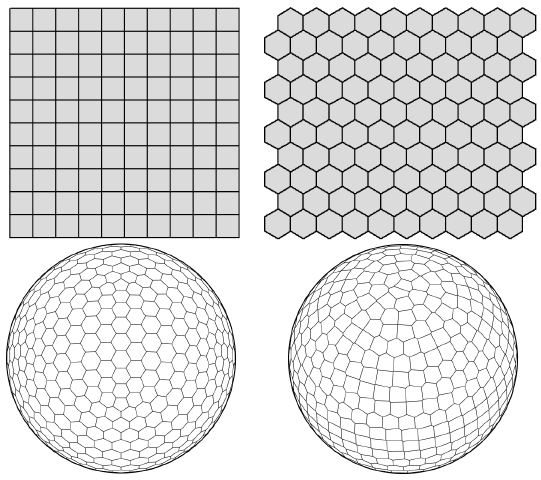
\includegraphics[width=0.75\linewidth]{topos.png}
  \end{figure}
  \end{center}
 \end{frame} 

\begin{frame}
	\frametitle{Data Generation}
 
\begin{block}{Synthetic Multivariate Data}
 \begin{itemize}
 \item  Follow Wu and Takatsuka (2006)
 \item  Seven clusters
 \item  Three dimension
 \item  Clusters are normally distributed w/ unit variance on each dimension
 \item  25,000 Observation -> 644 Neurons
 \end{itemize}
 \end{block} \end{frame} 

\begin{frame}
	\frametitle{Graph Based Implementation of SOM}
 
\begin{block}{Python}
 \begin{itemize}
 \item  Growing scientific community
 \item  Rapid development
 \end{itemize}
 \end{block} 
\begin{block}{Why}
 \begin{itemize}
 \item  Alternative topologies not available 
 \item  Difficult to extend
 \item  Flexibility over speed
 \begin{itemize}
 \item  SOM\_PAK: 90 seconds
 \item  PySOM: 45 minutes
 \end{itemize}
 \end{itemize}
 \end{block} 
\begin{block}{Graphs}
 \begin{itemize}
 \item  Topology independent
 \item  Flexible
 \end{itemize}
 \end{block} \end{frame} 


\section{Results} 

\subsection{Internal Heterogeneity vs. First-Order Neighborhood Size} 

\begin{frame}
	\frametitle{Diagnostic}
 
\begin{block}{Internal Heterogeneity vs. First-Order Neighborhood Size}
 \begin{itemize}
 \item  Does a neuron's I.H. decrease as its first-order neighborhood size increases?
 \begin{itemize}
 \item  Group neurons by degree and topology
 \item  Measure I.H. within each group
 \item  Check for difference of means and variance between groups
 \end{itemize}
 \end{itemize}
 \end{block} \end{frame} 

\begin{frame}
	\frametitle{Internal Heterogeneity vs. First-Order Neighborhood Size}
 
\begin{block}{Rectangular}
  \begin{center}
  \begin{figure}
  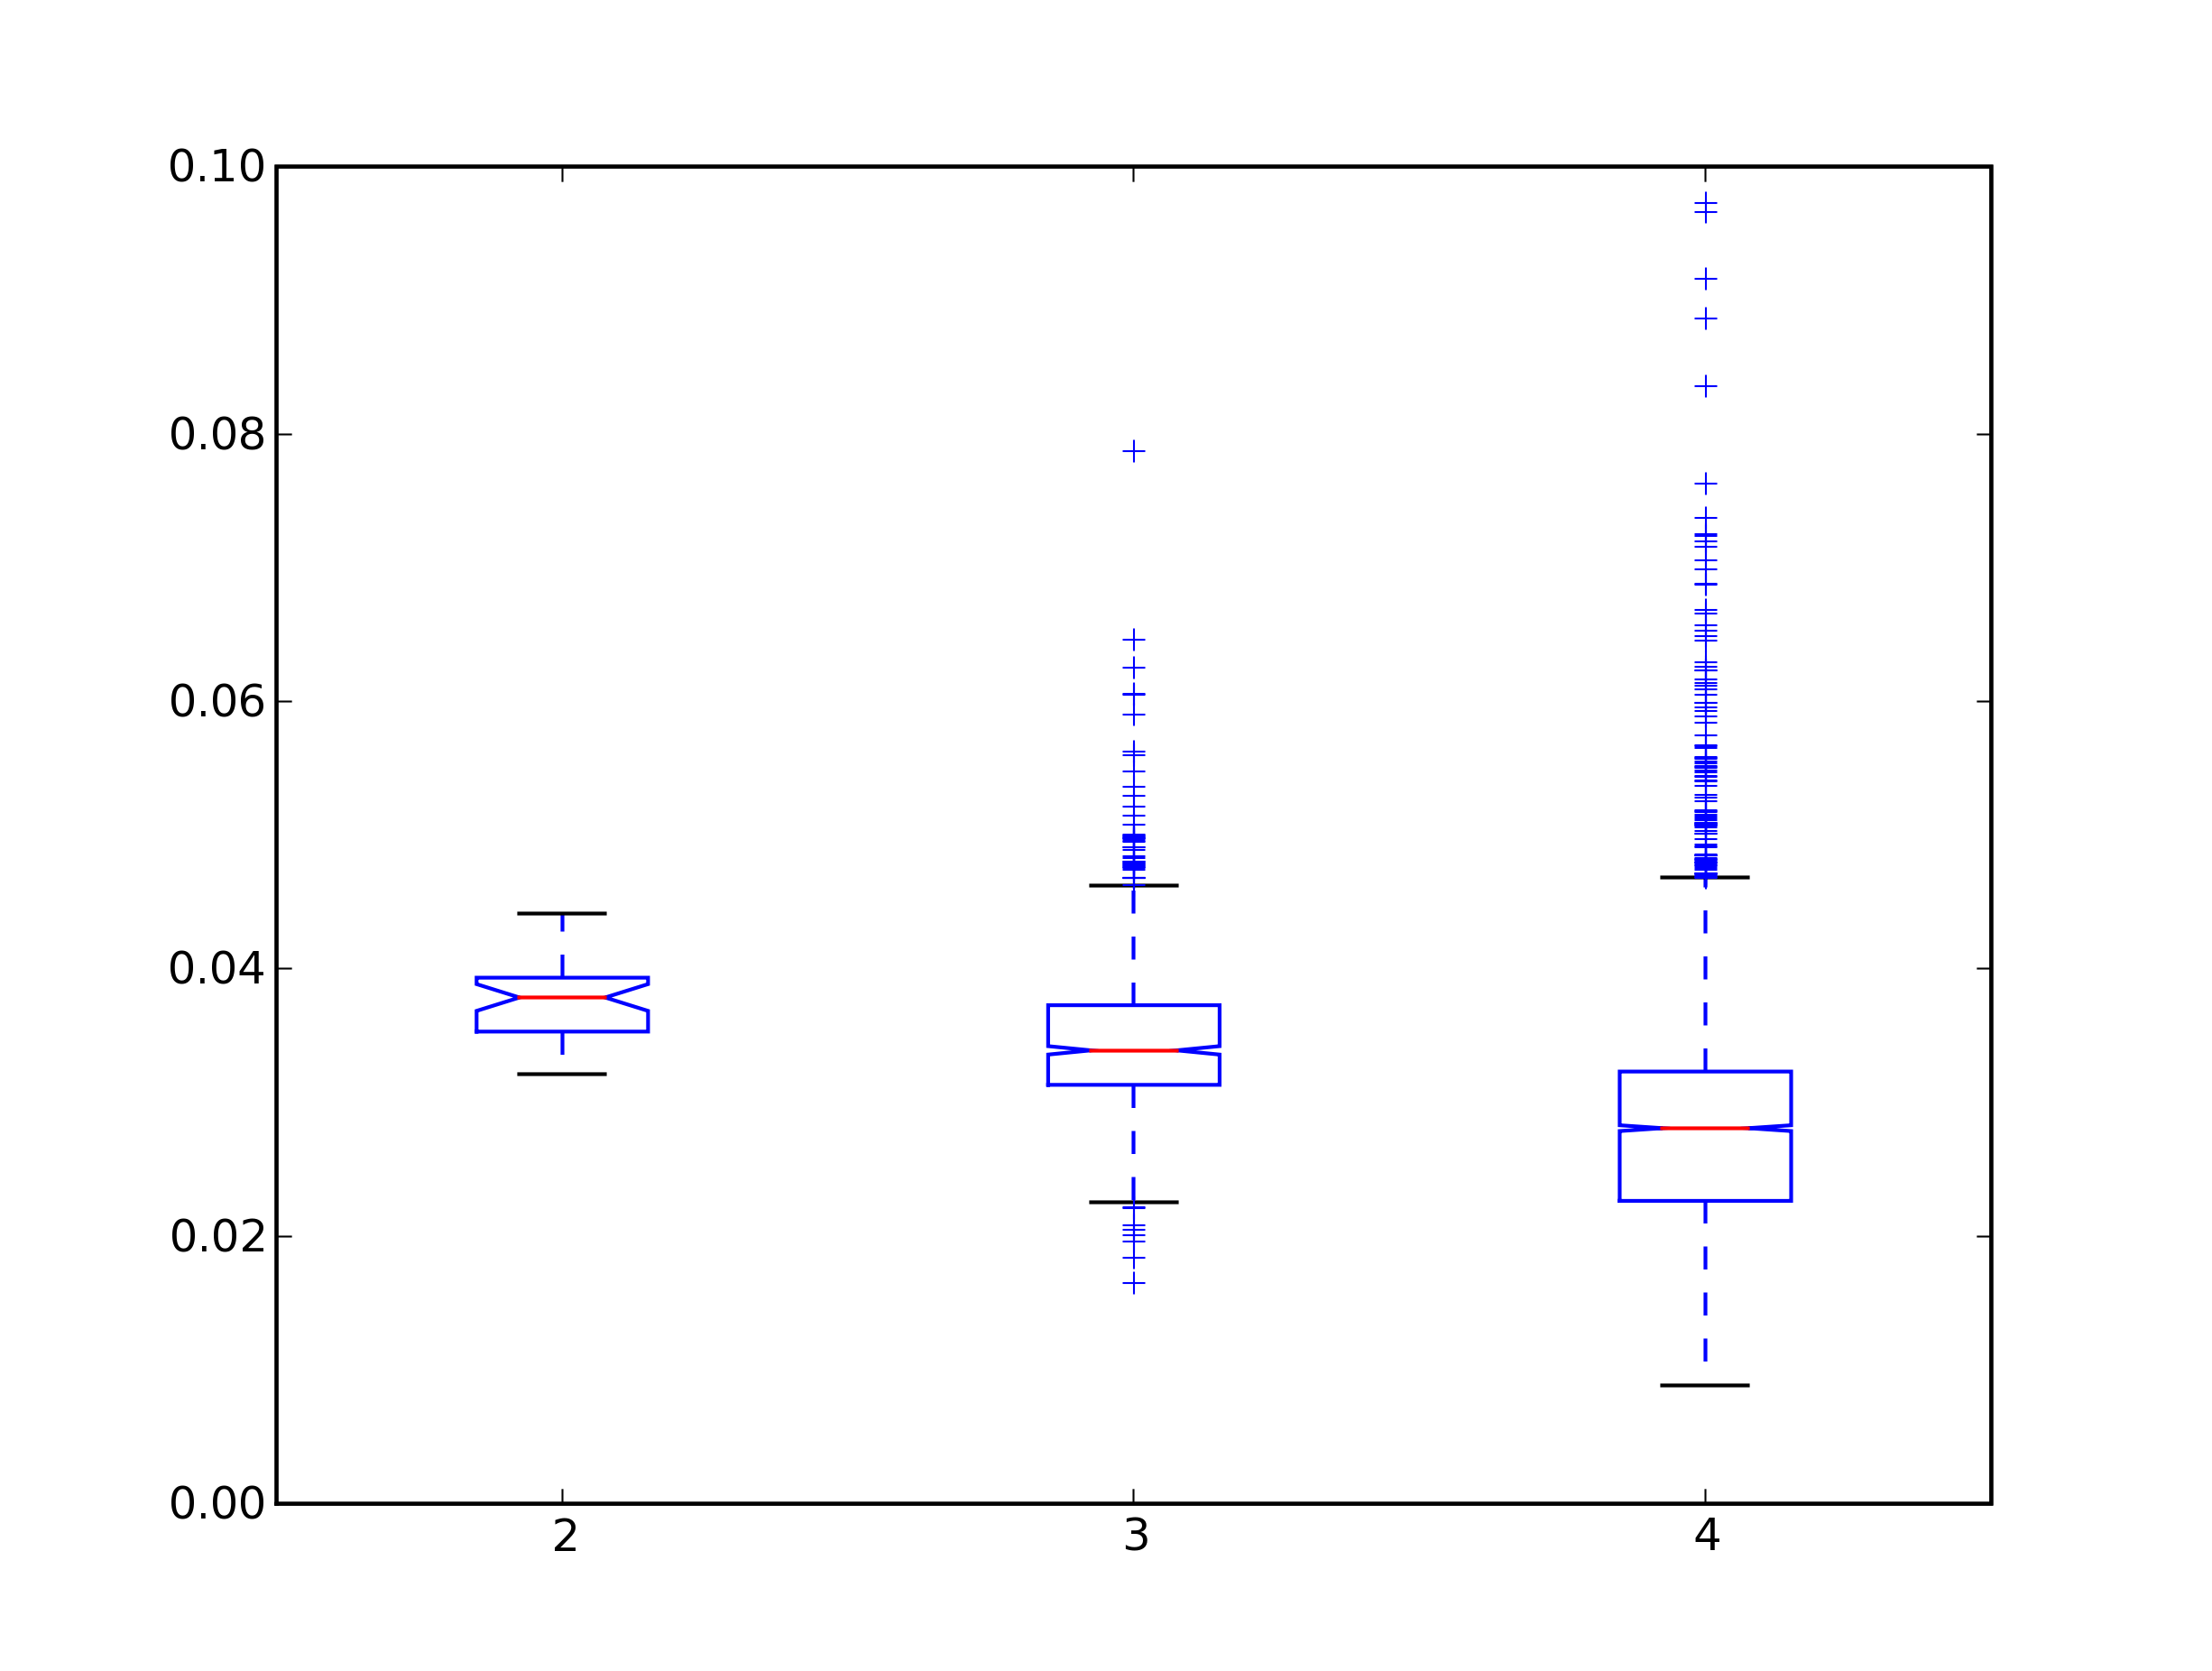
\includegraphics[width=0.75\linewidth]{rook_iv_box.png}
  \end{figure}
  \end{center}
 \end{block} \end{frame} 

\begin{frame}
	\frametitle{Internal Heterogeneity vs. First-Order Neighborhood Size}
 
\begin{block}{Hexagonal}
  \begin{center}
  \begin{figure}
  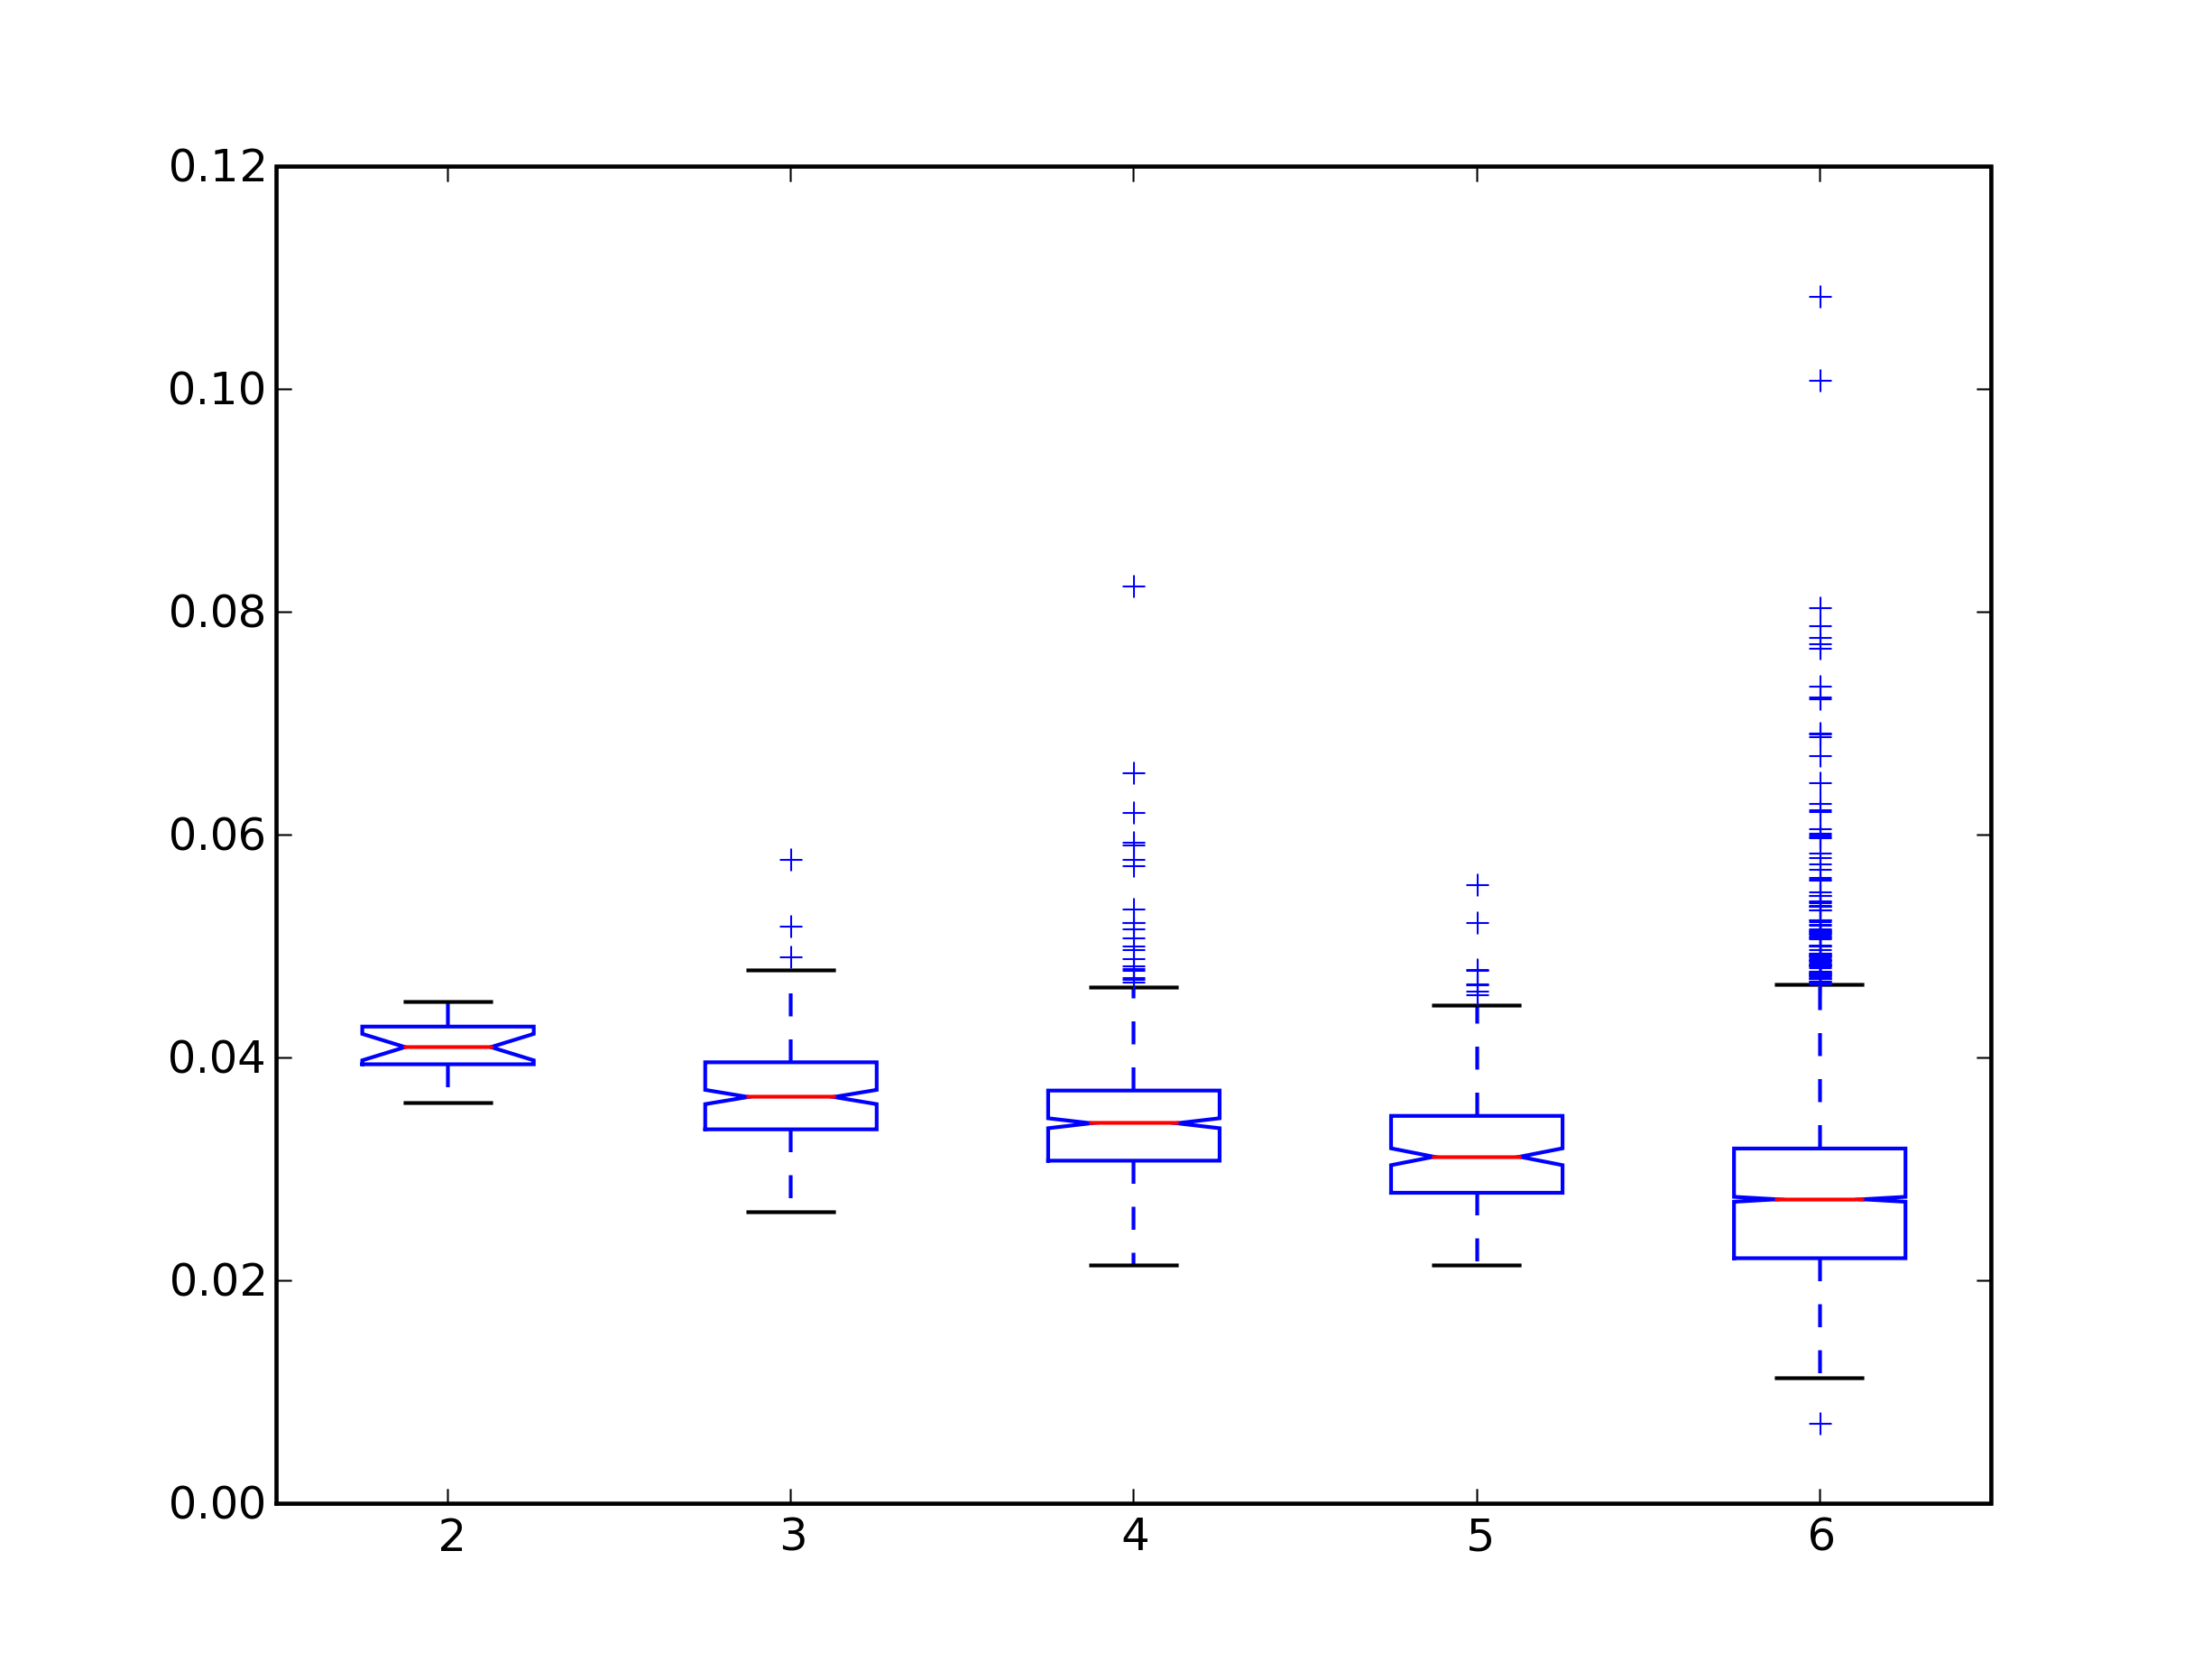
\includegraphics[width=0.75\linewidth]{hex_iv_box.png}
  \end{figure}
  \end{center}
 \end{block} \end{frame} 

\begin{frame}
	\frametitle{Internal Heterogeneity vs. First-Order Neighborhood Size}
 
\begin{block}{Geodesic}
  \begin{center}
  \begin{figure}
  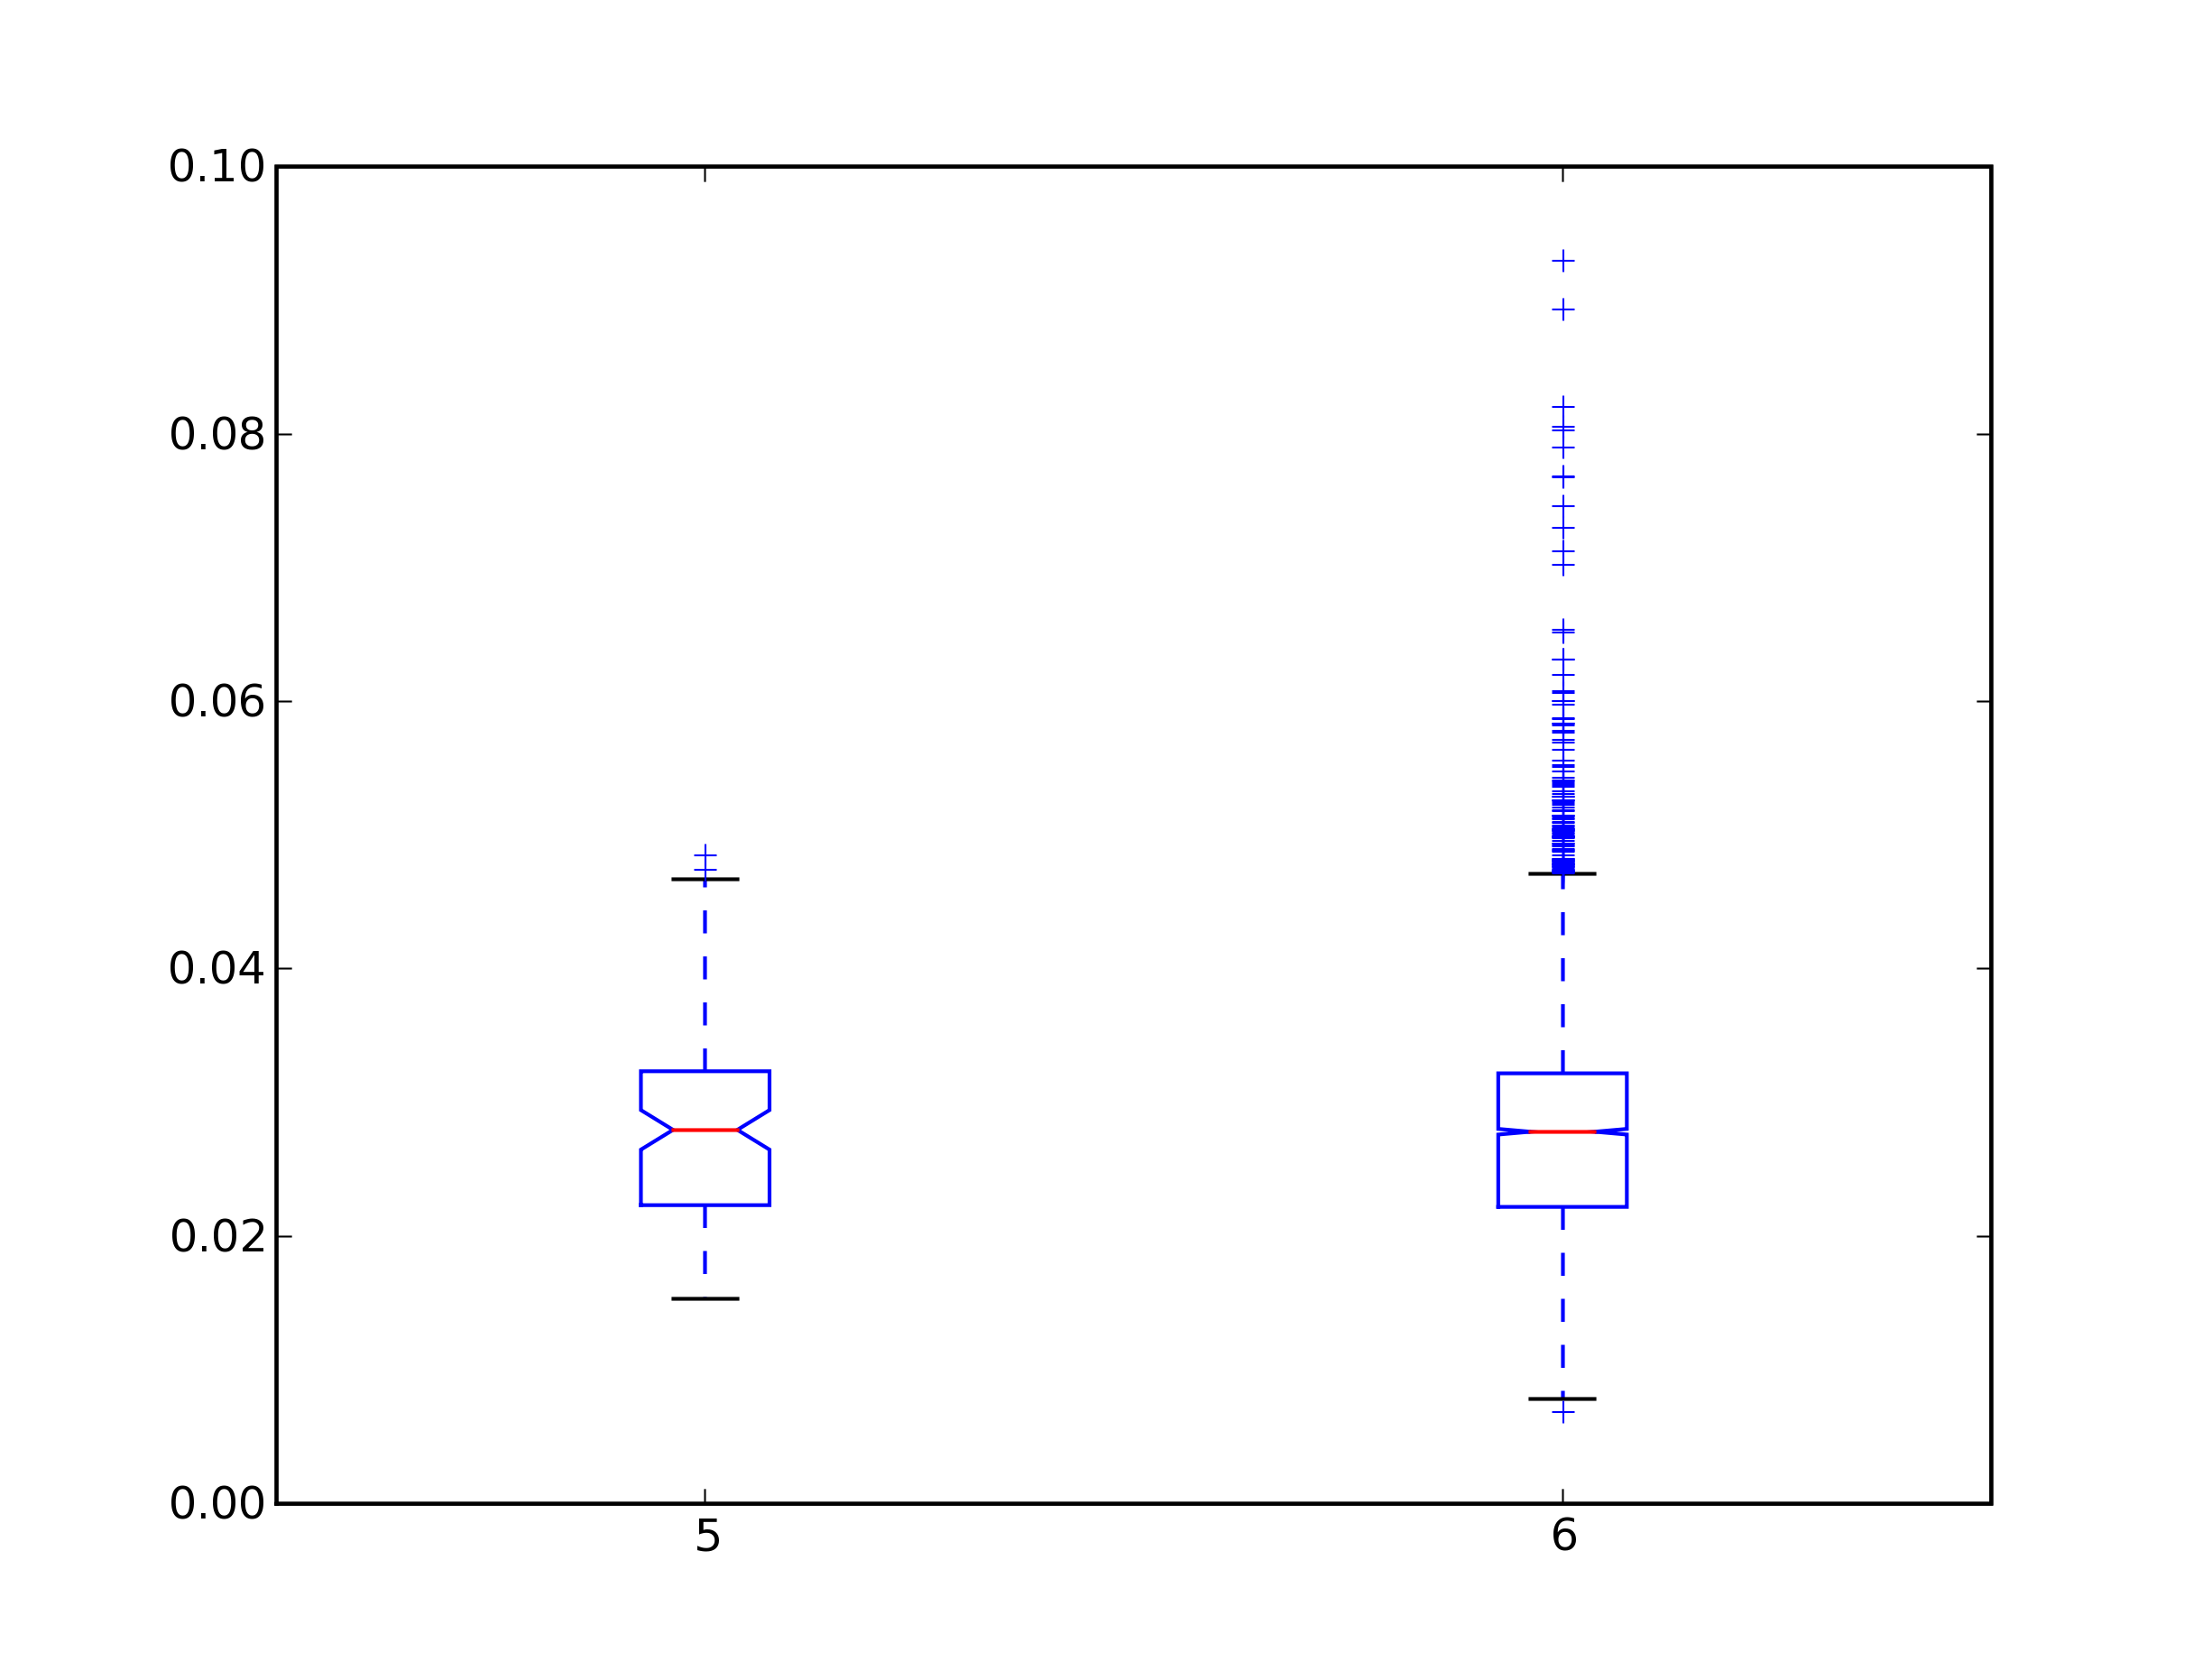
\includegraphics[width=0.75\linewidth]{geodesic_iv_box.png}
  \end{figure}
  \end{center}
 \end{block} \end{frame} 

\begin{frame}
	\frametitle{Internal Heterogeneity vs. First-Order Neighborhood Size}
 
\begin{block}{Spherical}
  \begin{center}
  \begin{figure}
  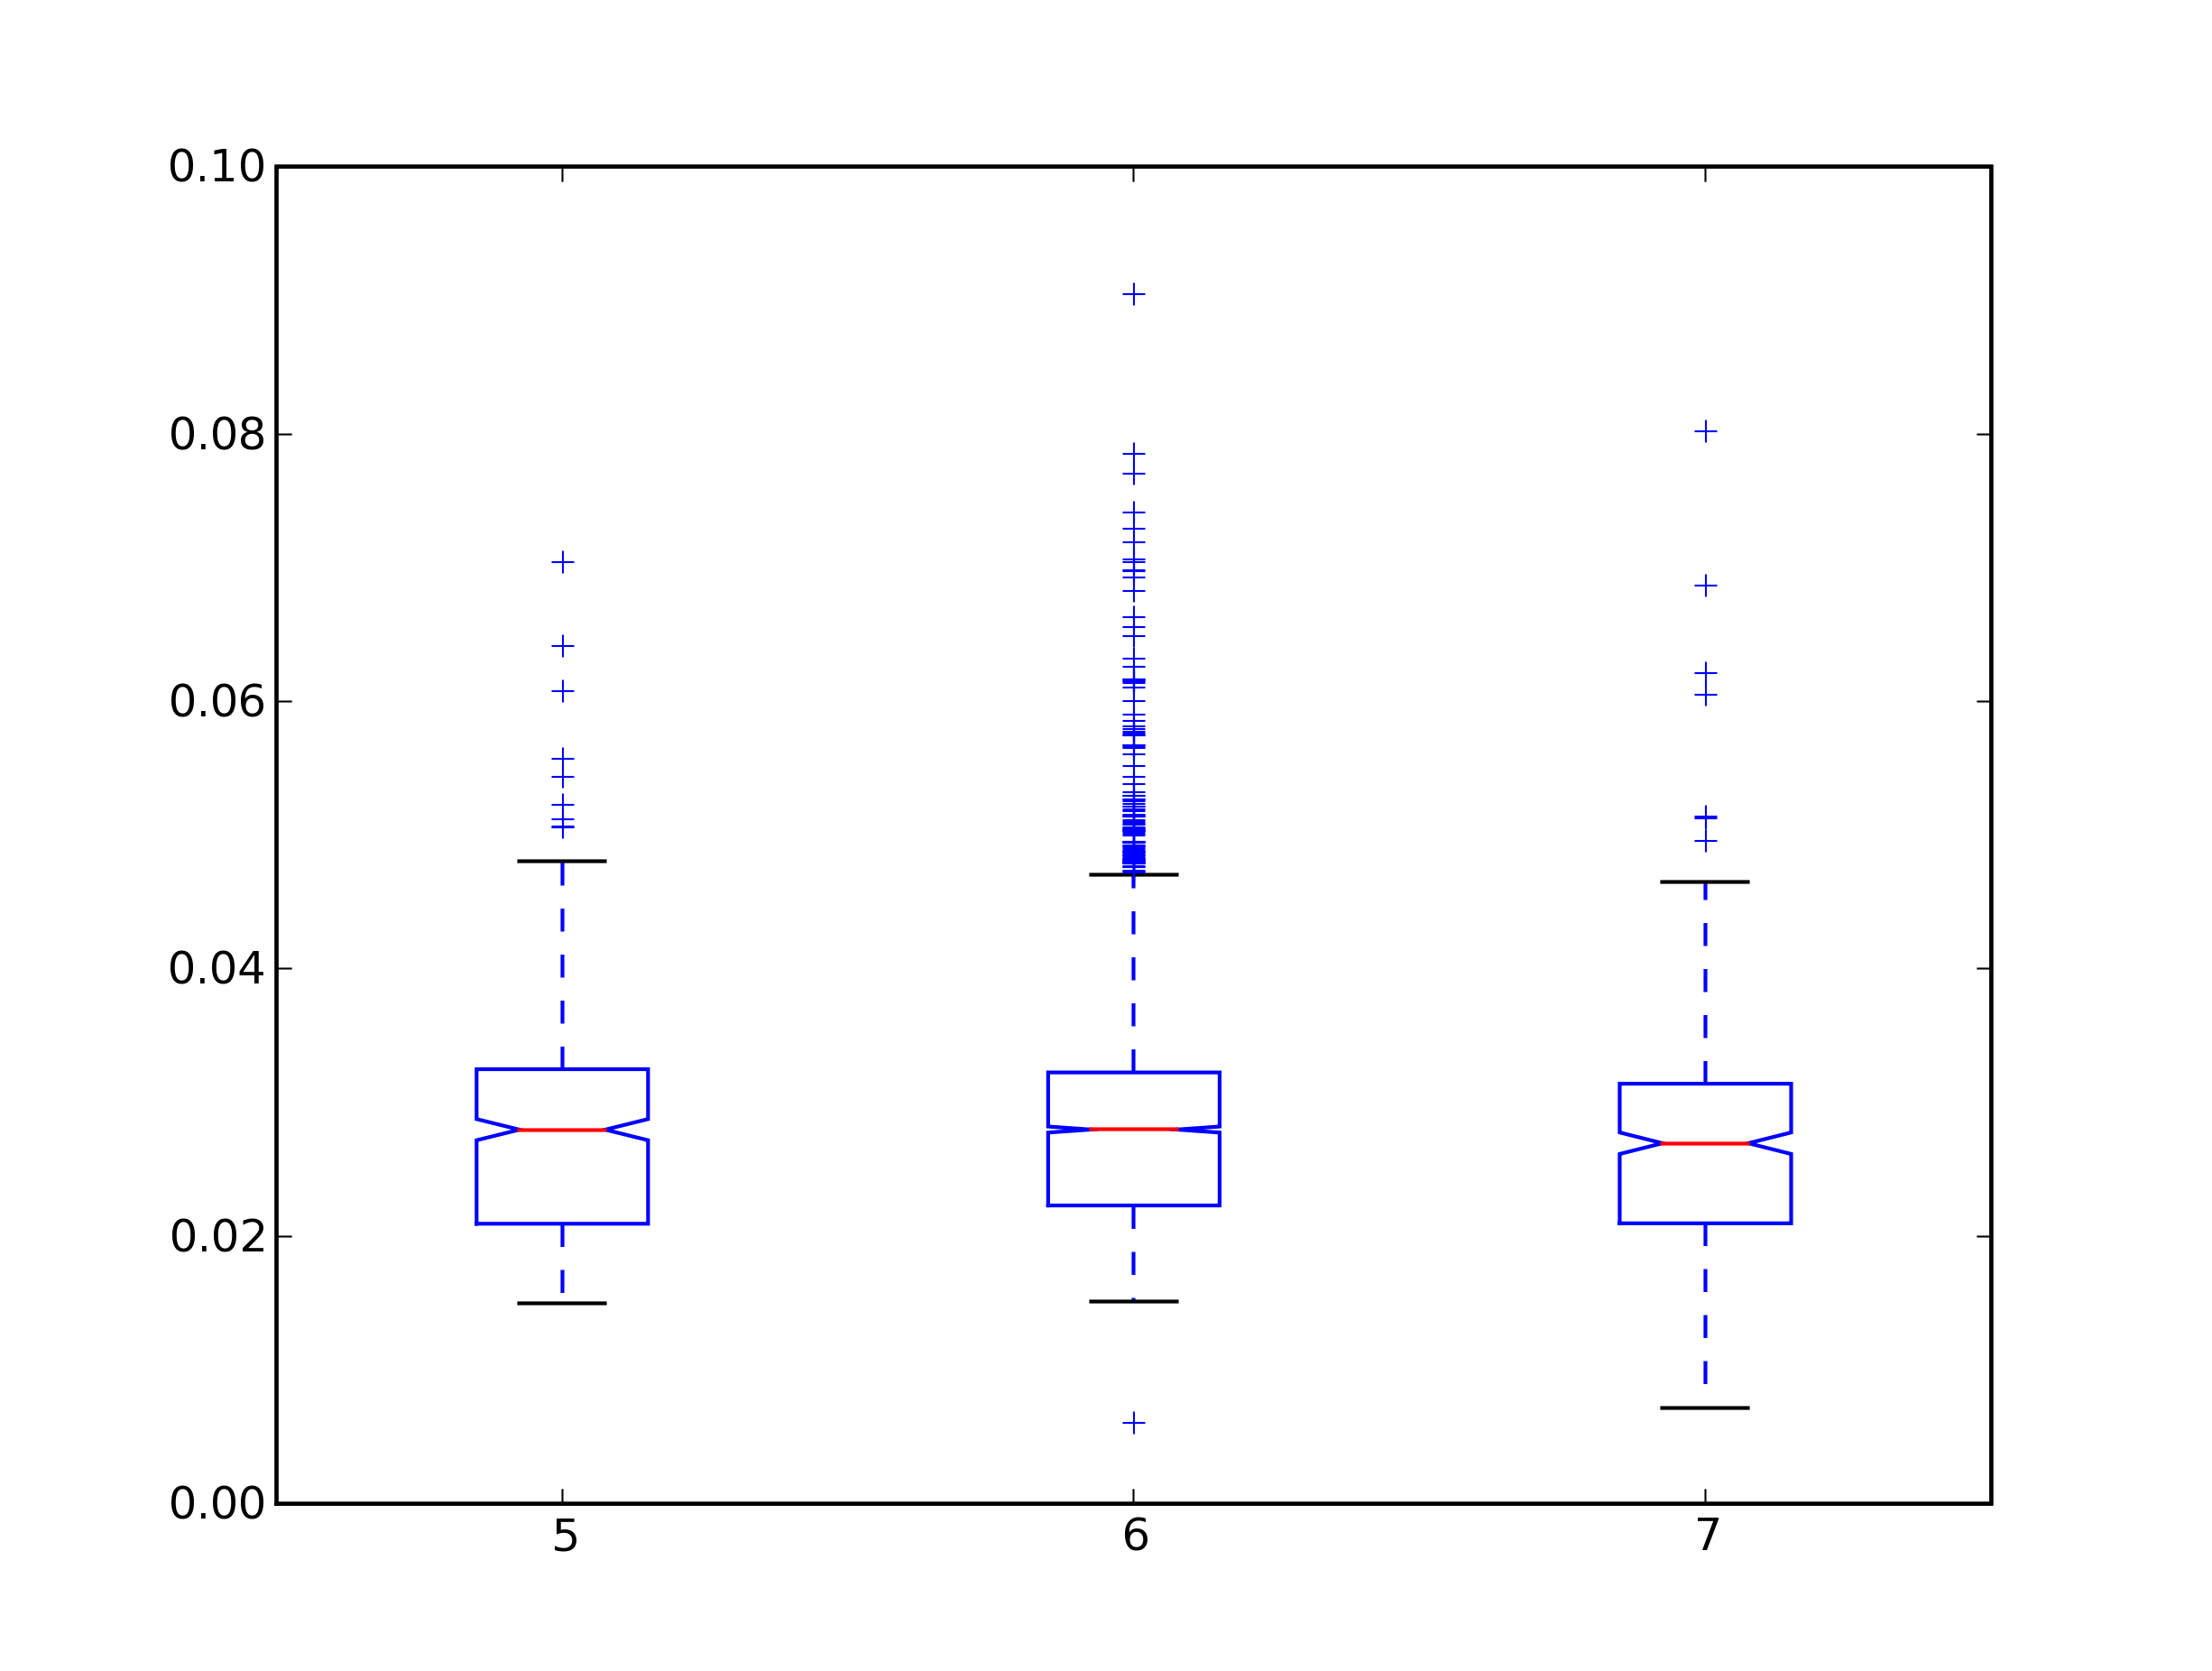
\includegraphics[width=0.75\linewidth]{graph_iv_box.png}
  \end{figure}
  \end{center}
 \end{block} \end{frame} 

\subsection{Internal Heterogeneity vs. Topological Regularity} 

\begin{frame}
	\frametitle{Diagnostic}
 
\begin{block}{Internal Heterogeneity vs. Topological Regularity}
 \begin{itemize}
 \item  Does a SOM's average I.H. increase in more irregular topologies?
 \begin{itemize}
 \item  Group neurons by Topology
 \item  Measure I.H. within each group
 \item  Check for difference of means and variance between groups
 \end{itemize}
 \end{itemize}
 \end{block} \end{frame} 

\begin{frame}
	\frametitle{Internal Heterogeneity vs. Topological Regularity}
  \begin{table}
  \centering
  \begin{minipage}{\textwidth}
  \caption{Measure of Topological Regularity and Sample Mean and Variance}
  \label{vardeg}
  \begin{tabular}{|c||c|c|c|}
  \hline
  &$c=1/n \sum_{i=1} (1/n \sum_{j=1} d_{i,j})^{-1}$&&\\
  Topology & Closeness Centrality & Mean & Variance\\
  \hline
  Rectangular & 0.0603 & 0.0294 &0.0001\\
  Hexagonal & 0.0739 & 0.0289 &0.0001\\
  Geodesic & 0.0890 & 0.0281 &0.0001\\
  Spherical & 0.0906 & 0.0281 &0.0001\\
  \hline
  \end{tabular}
  \end{minipage}
  \end{table}
 \end{frame} 

\begin{frame}
	\frametitle{Internal Heterogeneity vs. Topological Regularity}
  \begin{table}
    \begin{minipage}{\textwidth}
    \caption{Results of Difference of Mean Testing Across Topologies}
    \label{rlt:all}
    \begin{tabular}{|c||c|c|c|c|}
    \hline
    \textbf{Topology}&Rectangular&Hexagonal &Geodesic &Spherical\\\hline
    \hline
 	Rectangular & (0.000064) & \textbf{0.001000} & \textbf{0.000100} & \textbf{0.000100}\\\hline
 	Hexagonal & -0.000479 & (0.000064) & \textbf{0.000100} & \textbf{0.000100}\\\hline
 	Geodesic & -0.001329 & -0.000850 & (0.000060) & 0.505600\\\hline
 	Spherical & -0.001328 & -0.000849 & 0.000001 & (0.000061)\\\hline
    \end{tabular}
    \end{minipage}
  \end{table}
 \end{frame} 

\subsection{Visualization of Internal Heterogeneity} 

\begin{frame}
	\frametitle{Diagnostics}
 
\begin{block}{Visualization of Internal Heterogeneity}
 \begin{itemize}
 \item  What information can be learned from a mapping of the I.H.?
 \end{itemize}
 \end{block} \end{frame} 

\begin{frame}
	\frametitle{Visualization of Internal Heterogeneity}
 
\begin{block}{Rectangular}
  \begin{center}
  \begin{figure}
  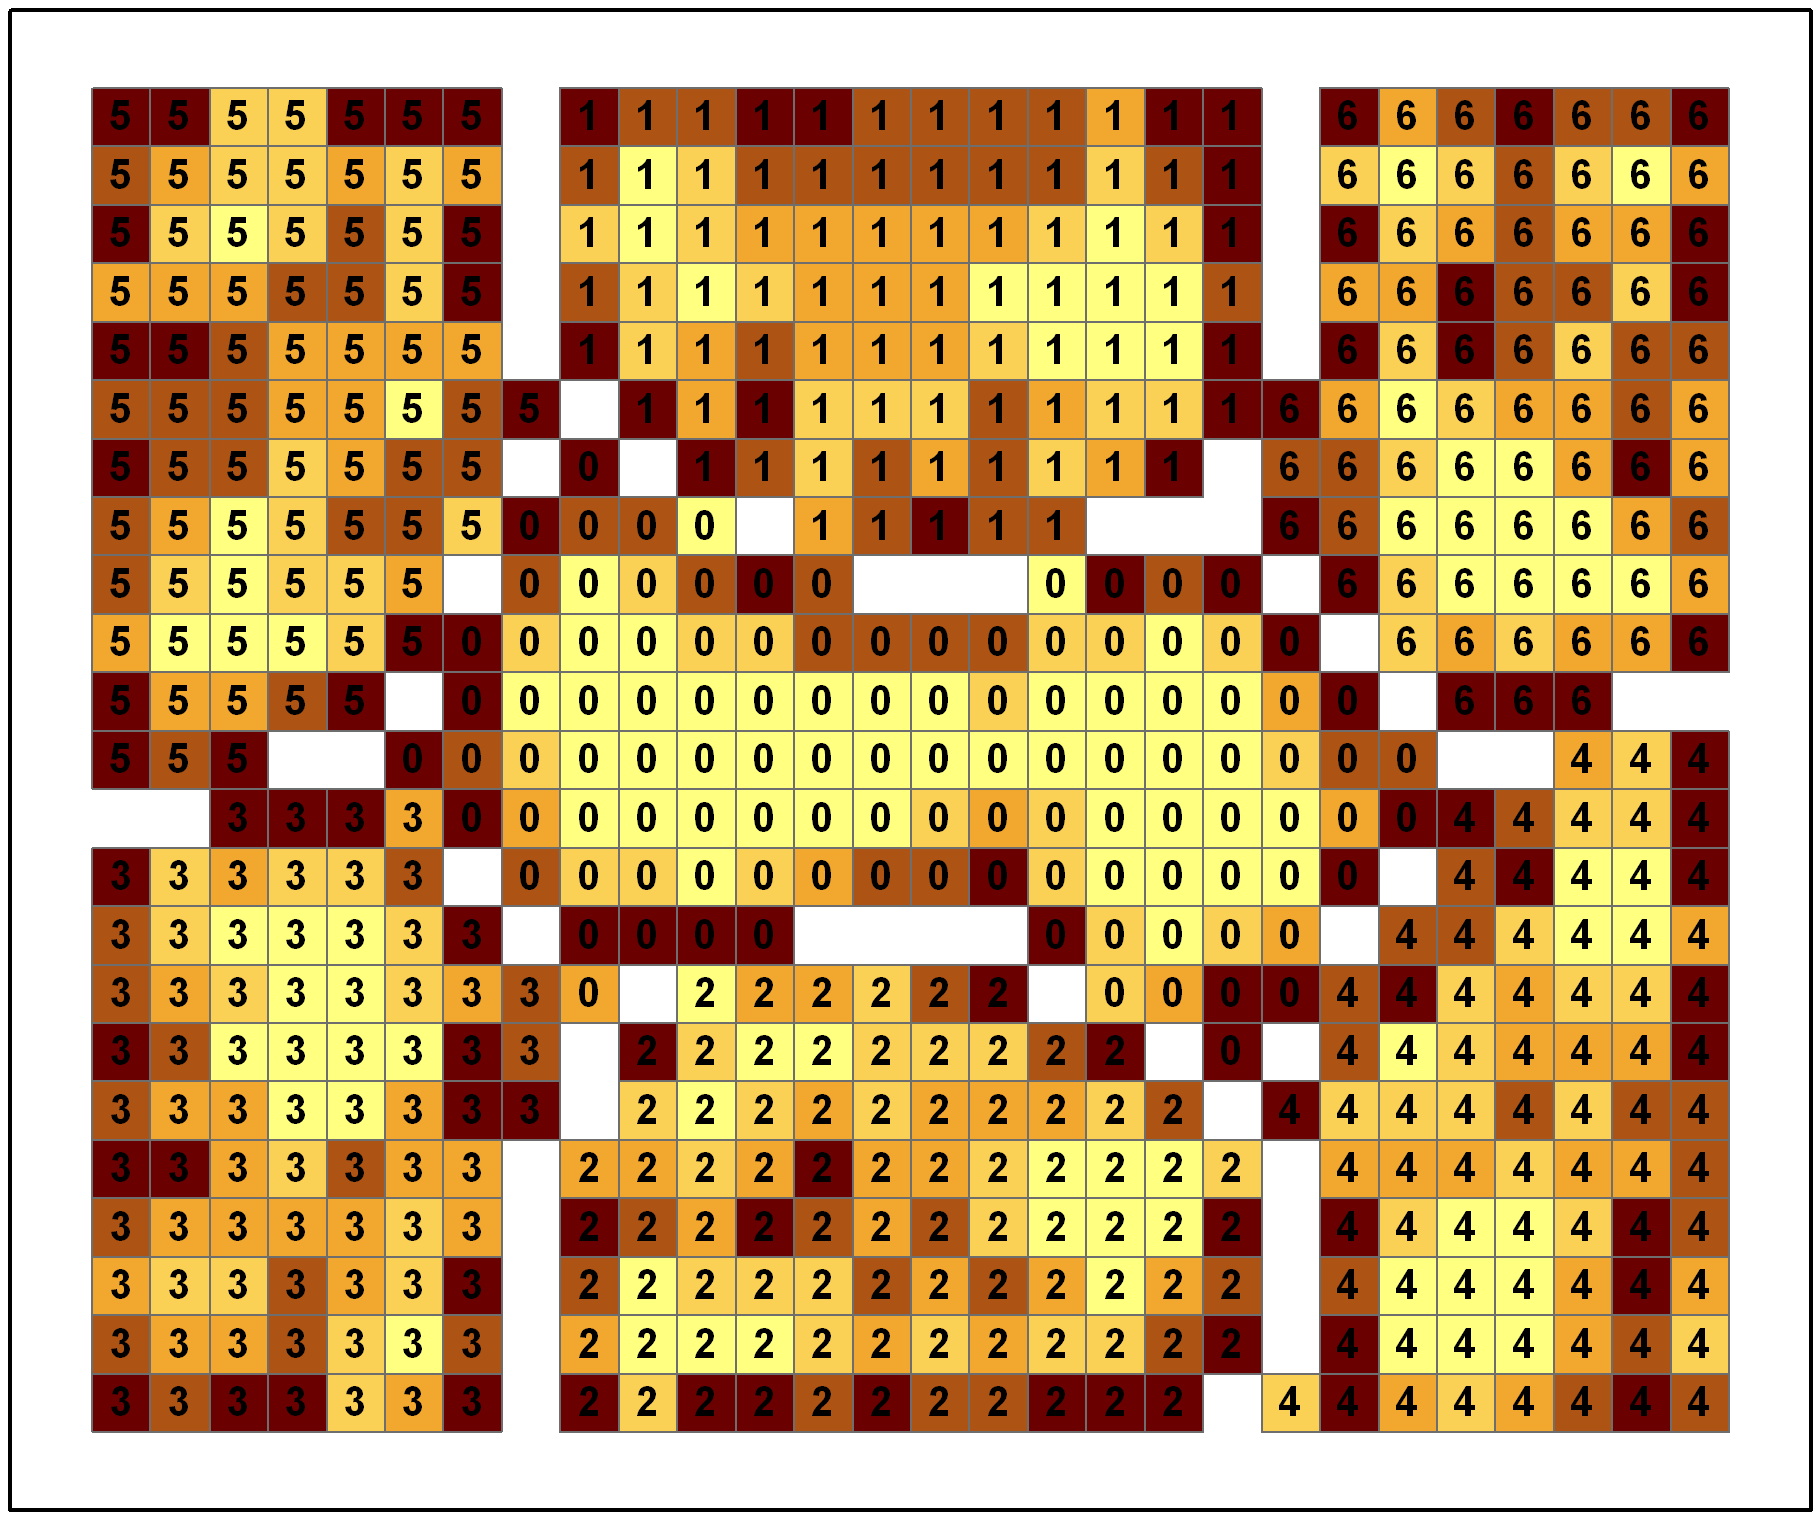
\includegraphics[width=0.70\linewidth]{rook_clusters.png}
  \end{figure}
  \end{center}
 \end{block} \end{frame} 

\begin{frame}
	\frametitle{Visualization of Internal Heterogeneity}
 
\begin{block}{Hexagonal}
  \begin{center}
  \begin{figure}
  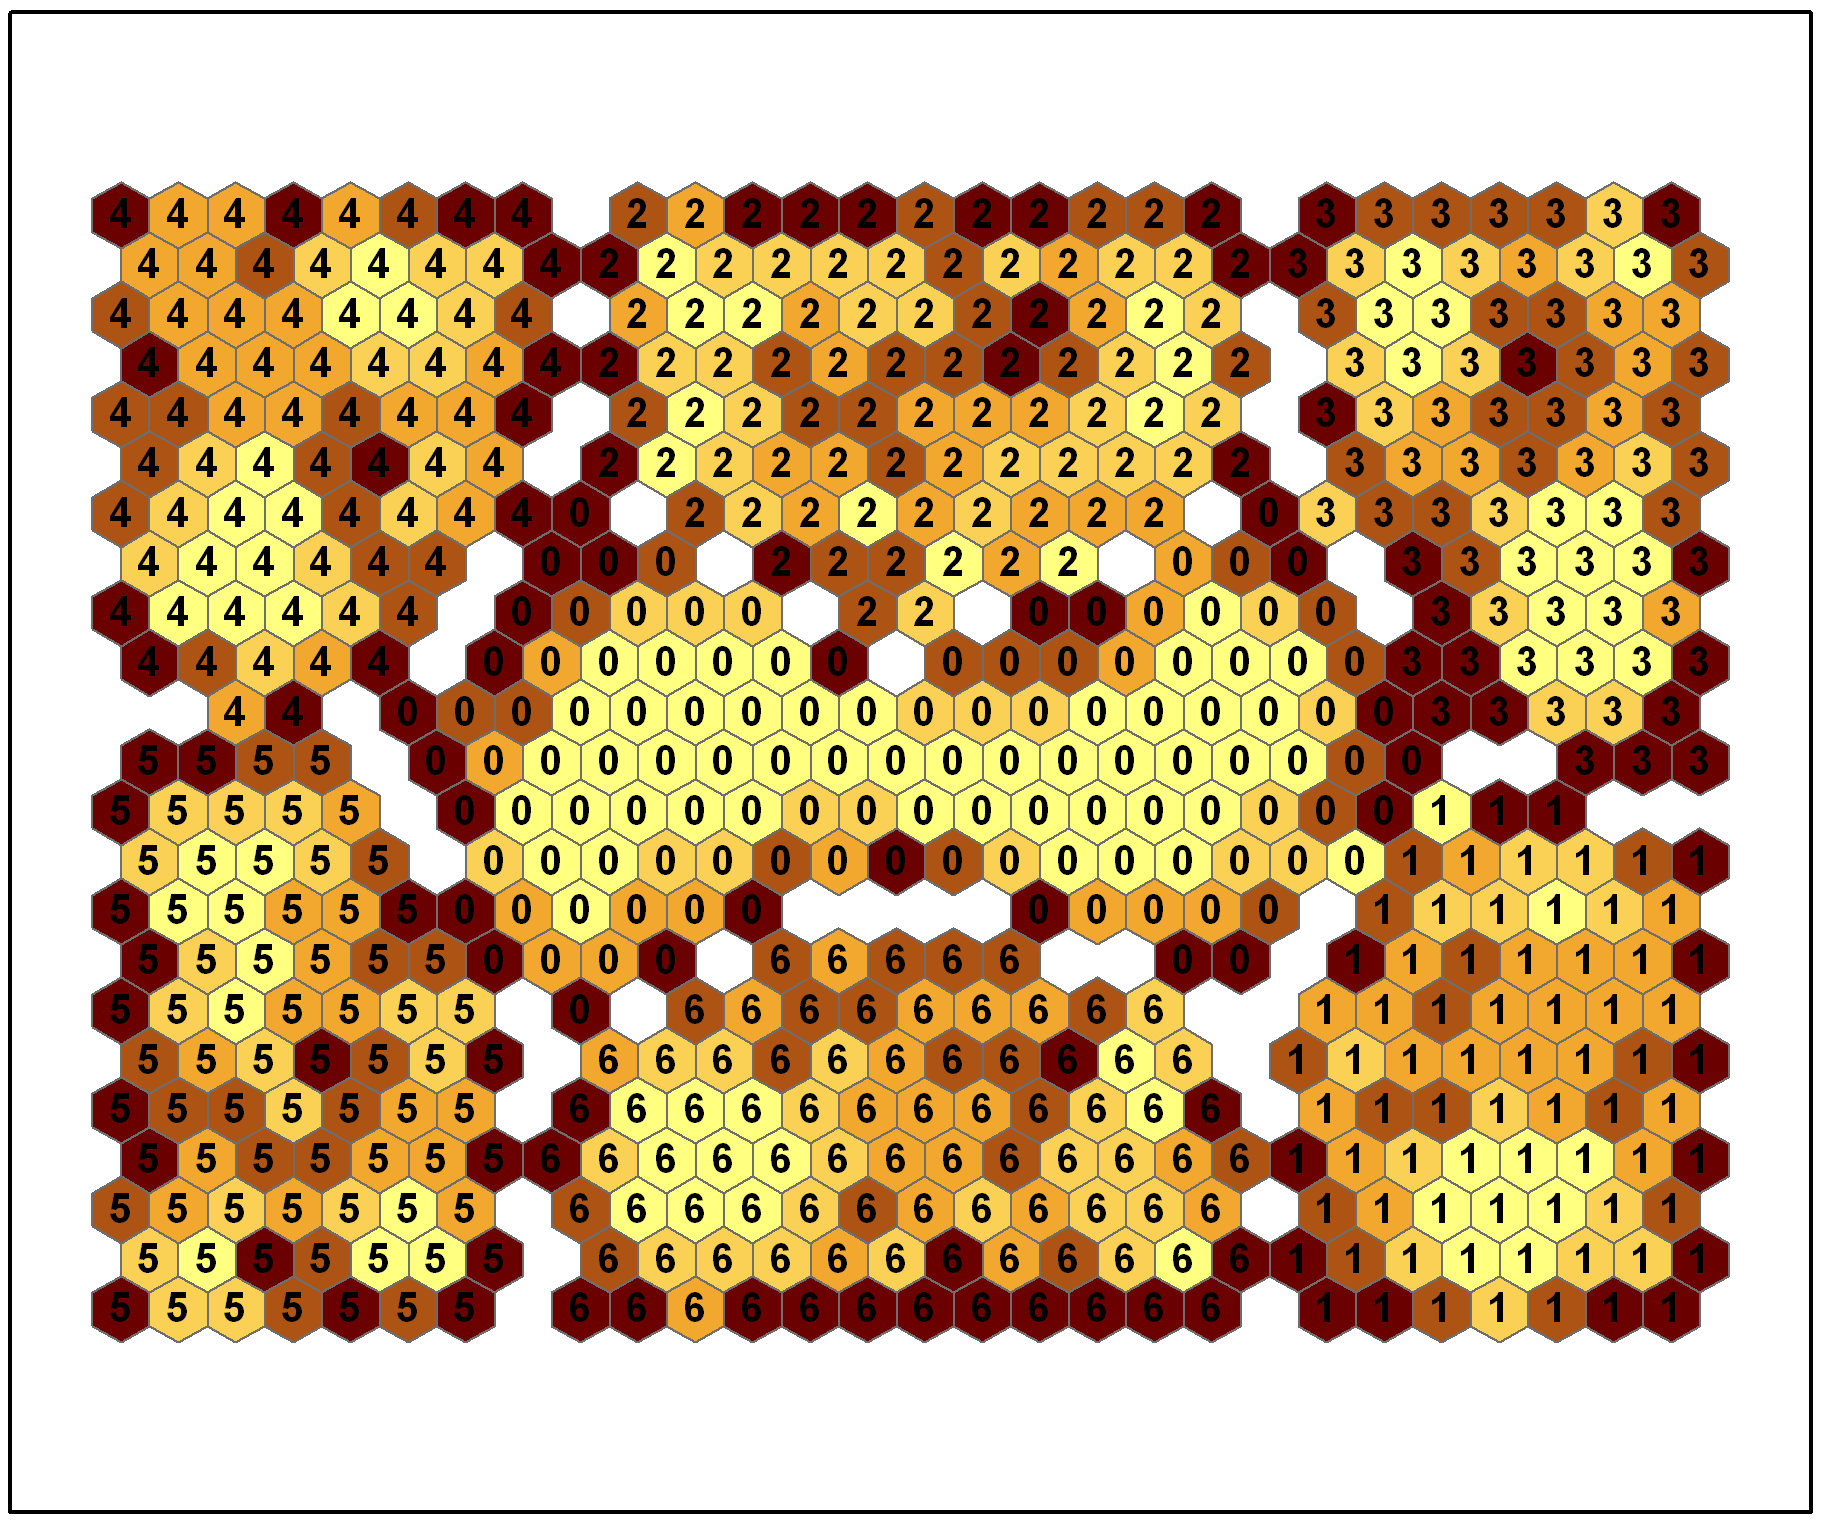
\includegraphics[width=0.70\linewidth]{hex_clusters.png}
  \end{figure}
  \end{center}
 \end{block} \end{frame} 

\begin{frame}
	\frametitle{Visualization of Internal Heterogeneity}
 
\begin{block}{Geodesic}
  \begin{center}
  \begin{figure}
  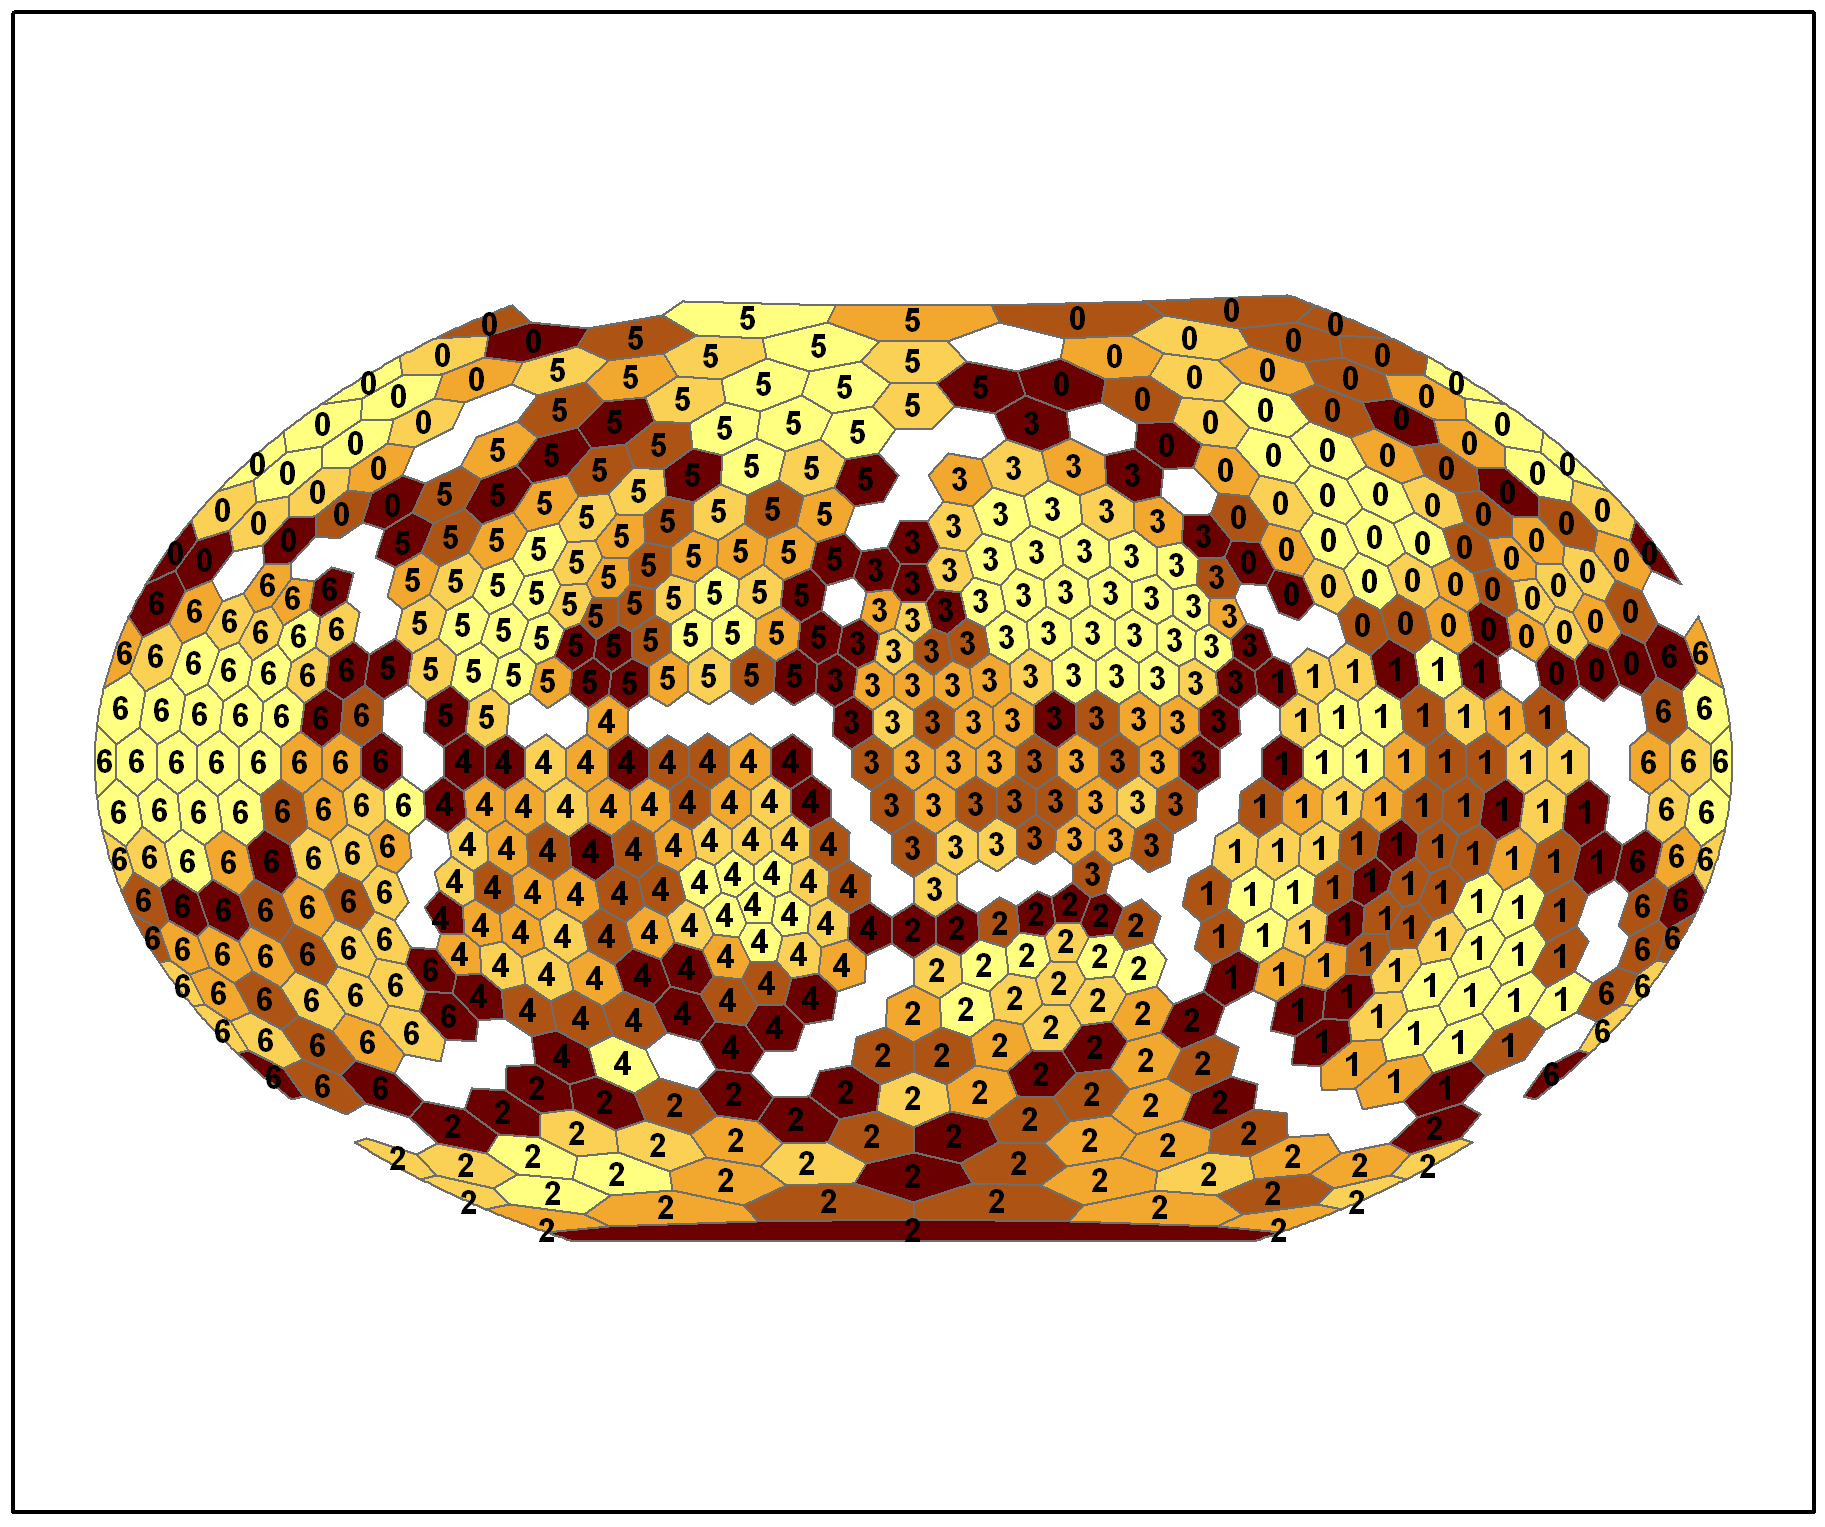
\includegraphics[width=0.70\linewidth]{geodesic_clusters.png}
  \end{figure}
  \end{center}
 \end{block} \end{frame} 

\begin{frame}
	\frametitle{Visualization of Internal Heterogeneity}
 
\begin{block}{Spherical}
  \begin{center}
  \begin{figure}
  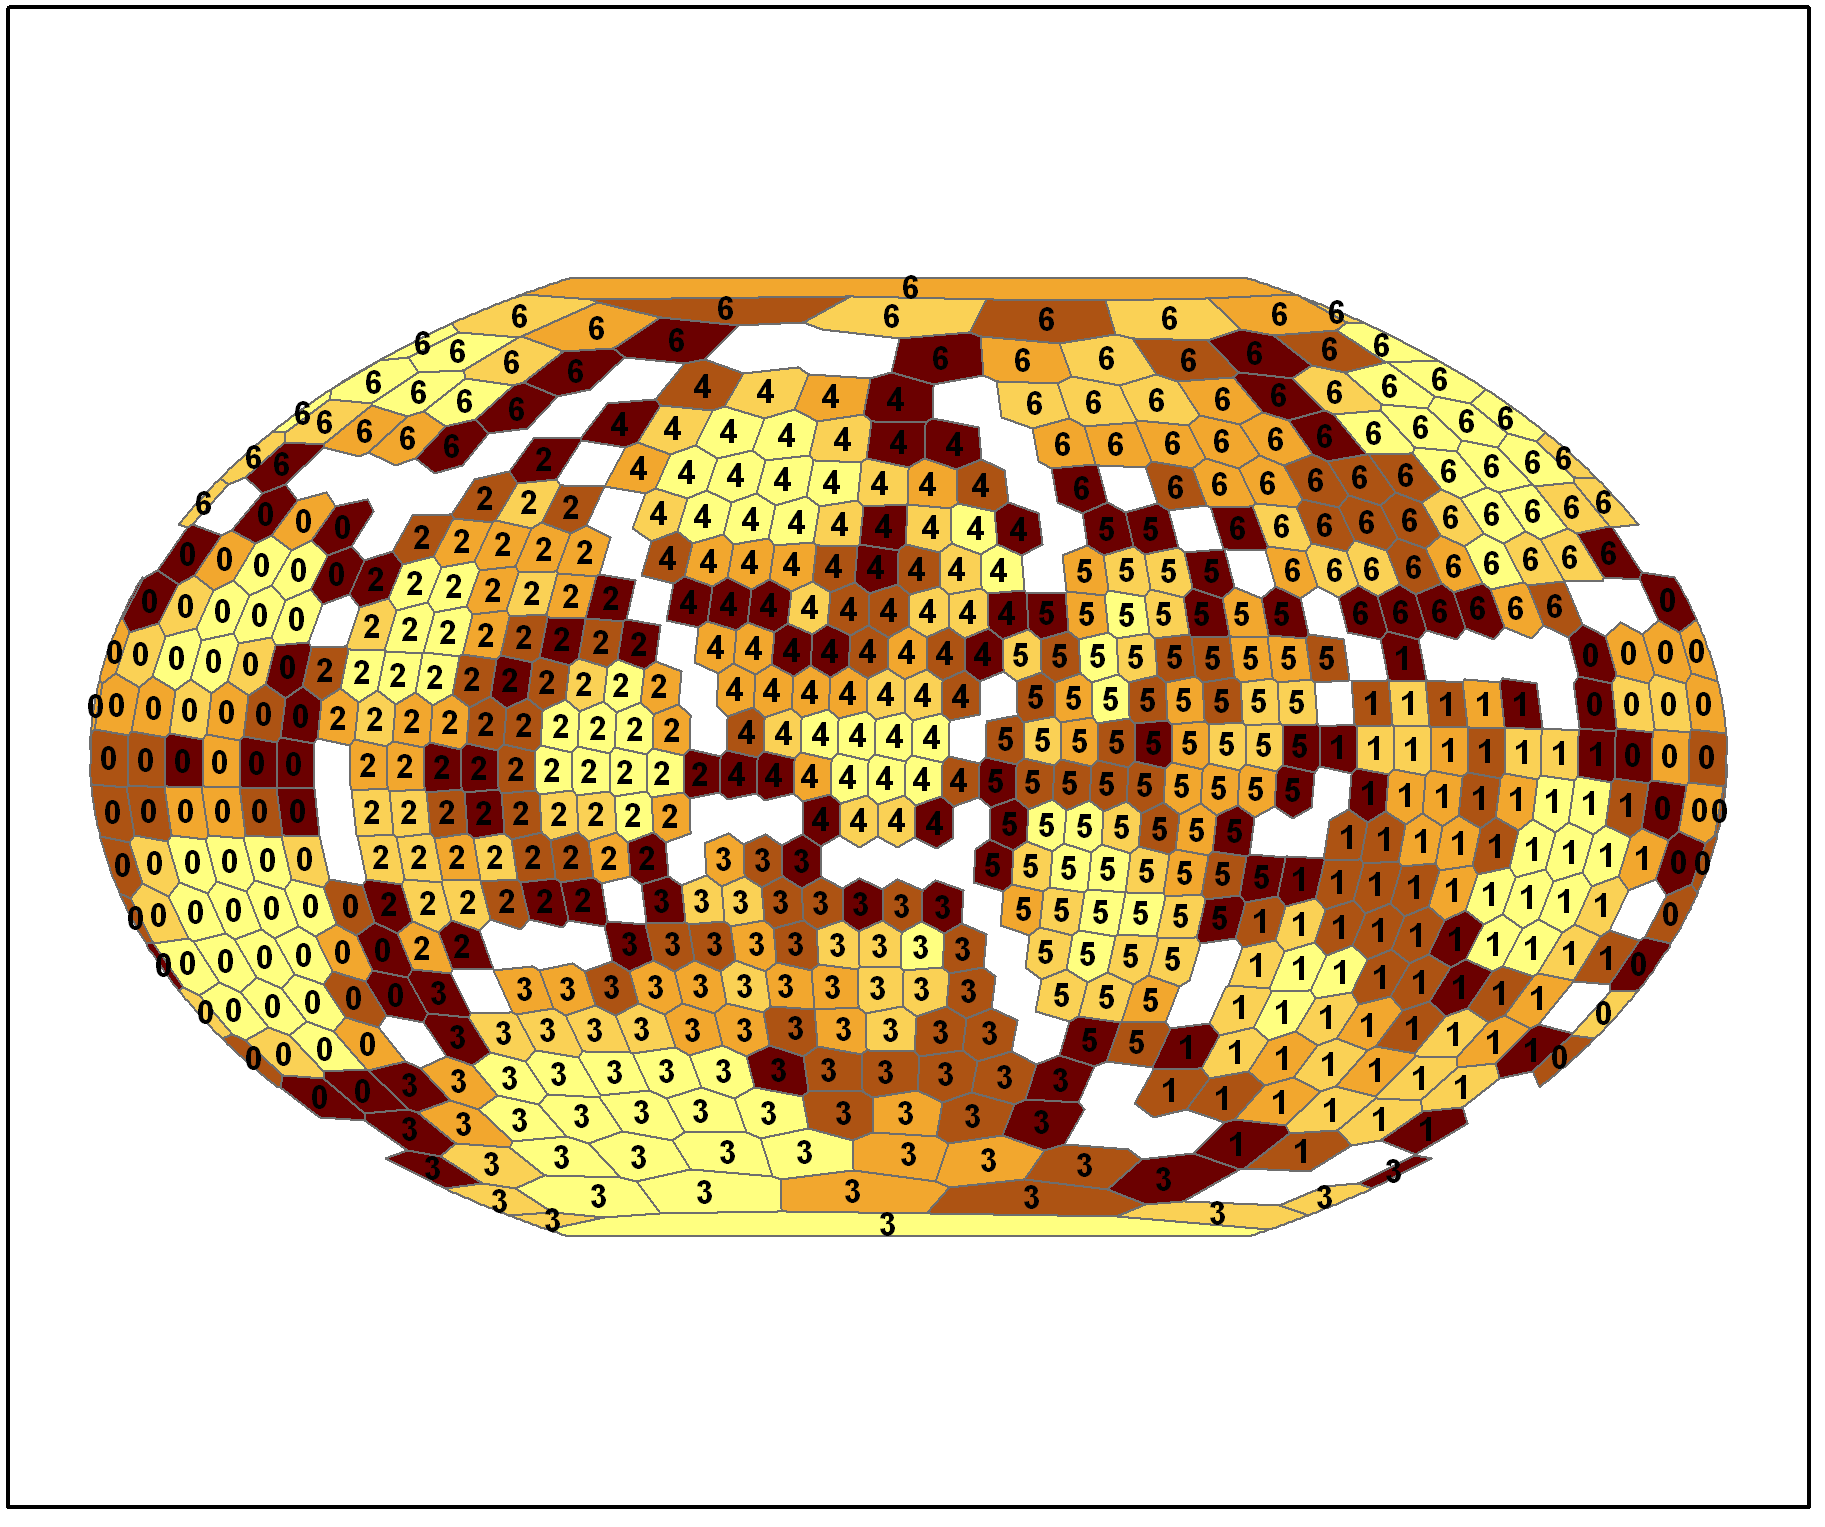
\includegraphics[width=0.70\linewidth]{sphere_clusters.png}
  \end{figure}
  \end{center}
 \end{block} \end{frame} 


\section{Conclusions} 

\subsection{Conclusions} 

\begin{frame}
	\frametitle{Key Findings}
 
\begin{block}{Internal Heterogeneity vs. First-Order Neighborhood Size}
 \begin{itemize}
 \item  Significant differences for hexagonal and rectangular topologies
 \item  One significant difference in spherical topology
 \begin{itemize}
 \item  Magnitude of difference very small compared with magnitudes in "flat" topologies
 \end{itemize}
 \item  No significant difference for geodesic
 \end{itemize}
 \end{block} 
\begin{block}{Internal Heterogeneity vs. Topological Regularity}
 \begin{itemize}
 \item  Geodesic and spherical show no significant differences
 \end{itemize}
 \end{block} 
\begin{block}{Visualization of Internal Heterogeneity}
 \begin{itemize}
 \item  Shows patterns of clustering
 \item  Provides insight into the self-organizing process
 \end{itemize}
 \end{block} \end{frame} 

\begin{frame}
	\frametitle{Objective}
 
\begin{block}{Question}
  Does Regularity Matter in Spherical SOM?
 \end{block} \end{frame} 

\begin{frame}
	\frametitle{Limitations}
 
\begin{block}{Qualifications}
 \begin{itemize}
 \item  Only addressing how topology effects the SOM.
 \begin{itemize}
 \item  Does not address the benefits of having or removing the edge.
 \item  Is pushing outliers to the edges a bad thing?
 \end{itemize}
 \end{itemize}
 \end{block} \end{frame} 

\begin{frame}
	\frametitle{Future Directions}
 
\begin{block}{Extensions}
 \begin{itemize}
 \item  Rotate sphere-based SOMs to show "central" feature
 \item  Compare different SOMs on more than just topology
 \item  Test other topologies
 \begin{itemize}
 \item  Remove nodes from the existing topologies
 \end{itemize}
 \end{itemize}
 \end{block} \end{frame} 

\begin{frame}
	\frametitle{Edge Effects in SOM}
  \begin{center}
  \begin{figure}
  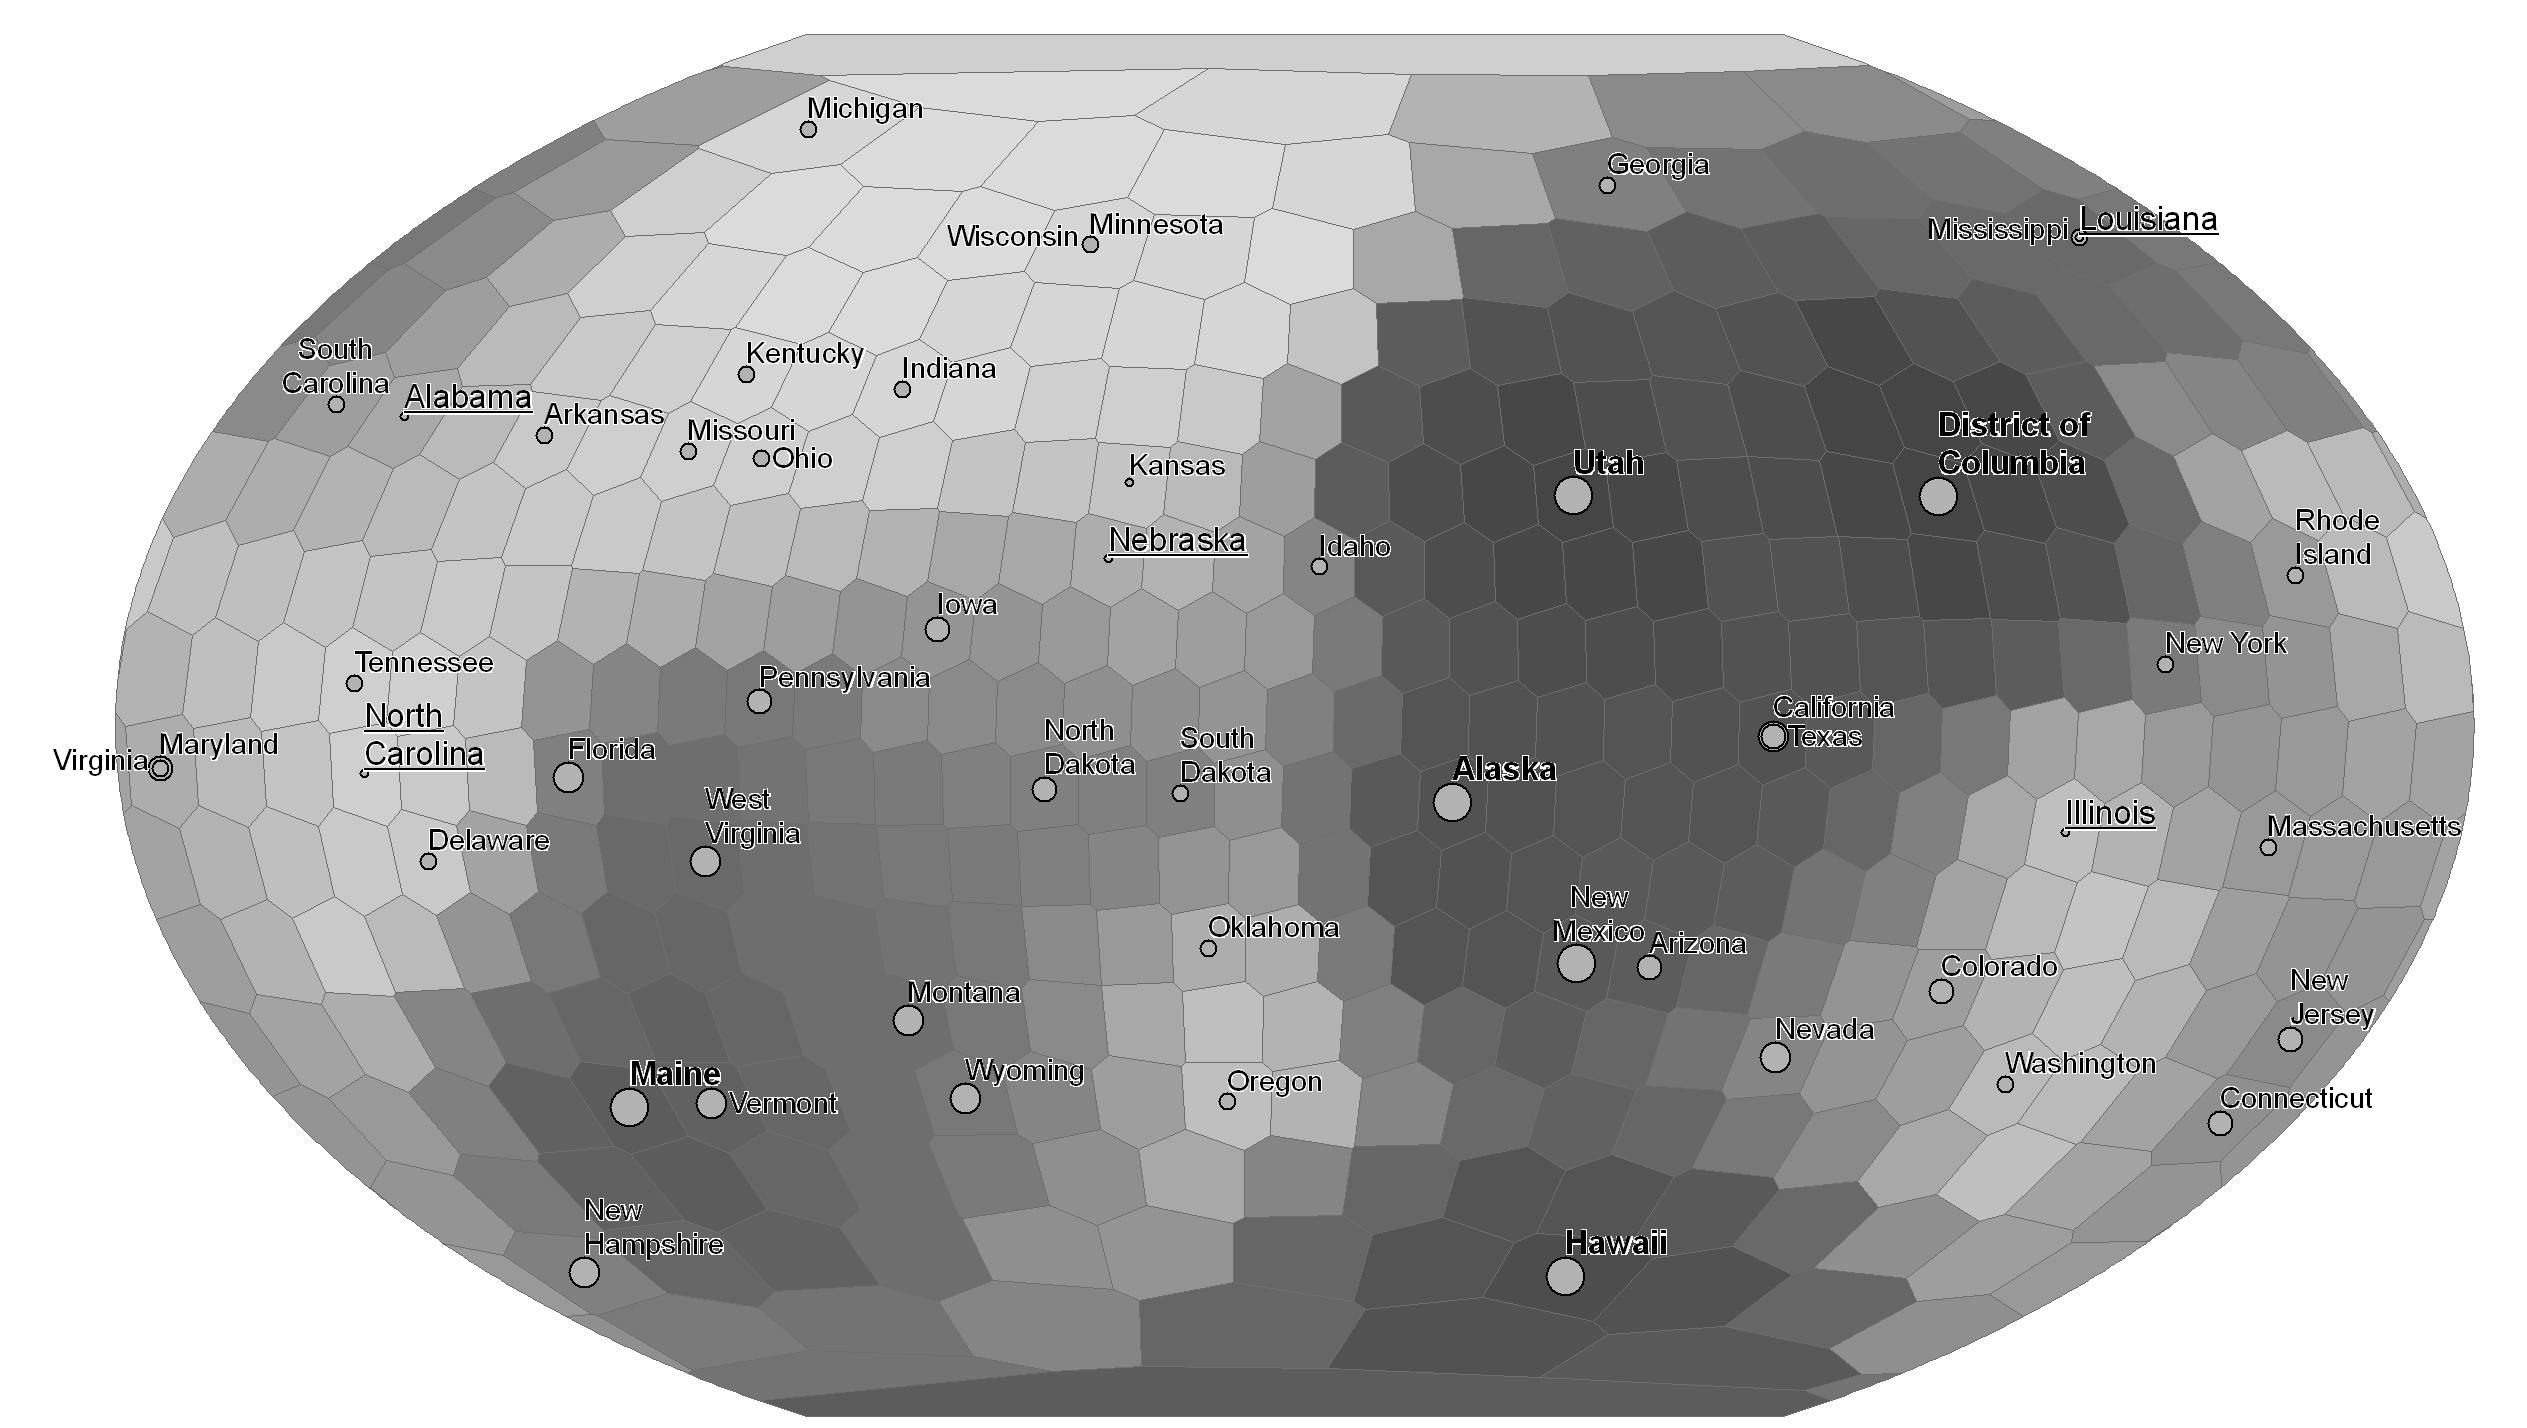
\includegraphics[width=\linewidth]{statesSphere.png}
  \end{figure}
  \end{center}
 \end{frame}
\end{document}
